% Options for packages loaded elsewhere
\PassOptionsToPackage{unicode}{hyperref}
\PassOptionsToPackage{hyphens}{url}
%
\documentclass[
]{article}
\usepackage{amsmath,amssymb}
\usepackage{iftex}
\ifPDFTeX
  \usepackage[T1]{fontenc}
  \usepackage[utf8]{inputenc}
  \usepackage{textcomp} % provide euro and other symbols
\else % if luatex or xetex
  \usepackage{unicode-math} % this also loads fontspec
  \defaultfontfeatures{Scale=MatchLowercase}
  \defaultfontfeatures[\rmfamily]{Ligatures=TeX,Scale=1}
\fi
\usepackage{lmodern}
\ifPDFTeX\else
  % xetex/luatex font selection
\fi
% Use upquote if available, for straight quotes in verbatim environments
\IfFileExists{upquote.sty}{\usepackage{upquote}}{}
\IfFileExists{microtype.sty}{% use microtype if available
  \usepackage[]{microtype}
  \UseMicrotypeSet[protrusion]{basicmath} % disable protrusion for tt fonts
}{}
\makeatletter
\@ifundefined{KOMAClassName}{% if non-KOMA class
  \IfFileExists{parskip.sty}{%
    \usepackage{parskip}
  }{% else
    \setlength{\parindent}{0pt}
    \setlength{\parskip}{6pt plus 2pt minus 1pt}}
}{% if KOMA class
  \KOMAoptions{parskip=half}}
\makeatother
\usepackage{xcolor}
\usepackage[margin=1in]{geometry}
\usepackage{longtable,booktabs,array}
\usepackage{calc} % for calculating minipage widths
% Correct order of tables after \paragraph or \subparagraph
\usepackage{etoolbox}
\makeatletter
\patchcmd\longtable{\par}{\if@noskipsec\mbox{}\fi\par}{}{}
\makeatother
% Allow footnotes in longtable head/foot
\IfFileExists{footnotehyper.sty}{\usepackage{footnotehyper}}{\usepackage{footnote}}
\makesavenoteenv{longtable}
\usepackage{graphicx}
\makeatletter
\def\maxwidth{\ifdim\Gin@nat@width>\linewidth\linewidth\else\Gin@nat@width\fi}
\def\maxheight{\ifdim\Gin@nat@height>\textheight\textheight\else\Gin@nat@height\fi}
\makeatother
% Scale images if necessary, so that they will not overflow the page
% margins by default, and it is still possible to overwrite the defaults
% using explicit options in \includegraphics[width, height, ...]{}
\setkeys{Gin}{width=\maxwidth,height=\maxheight,keepaspectratio}
% Set default figure placement to htbp
\makeatletter
\def\fps@figure{htbp}
\makeatother
\setlength{\emergencystretch}{3em} % prevent overfull lines
\providecommand{\tightlist}{%
  \setlength{\itemsep}{0pt}\setlength{\parskip}{0pt}}
\setcounter{secnumdepth}{-\maxdimen} % remove section numbering
\usepackage{fontspec}
\setmainfont{NanumGothic}
\ifLuaTeX
  \usepackage{selnolig}  % disable illegal ligatures
\fi
\usepackage{bookmark}
\IfFileExists{xurl.sty}{\usepackage{xurl}}{} % add URL line breaks if available
\urlstyle{same}
\hypersetup{
  pdftitle={Quiz 250414 (Wason Selection Task)},
  pdfauthor={coop711},
  hidelinks,
  pdfcreator={LaTeX via pandoc}}

\title{Quiz 250414 (Wason Selection Task)}
\author{coop711}
\date{2025-04-14}

\begin{document}
\maketitle

\section{7주차 데이터 실험
집계}\label{uxc8fcuxcc28-uxb370uxc774uxd130-uxc2e4uxd5d8-uxc9d1uxacc4}

\subsection{실험의 목적}\label{uxc2e4uxd5d8uxc758-uxbaa9uxc801}

7주차 구글 예습 설문지 집계결과를 분석합니다.

Q1 \textasciitilde{} Q6에서는 랜덤화의 효과로 Red, Black 이 얼마나
닮았는지 알아봅니다.

Q7에서는 Wason Selection Task에서 추상적 문제에 취약하고 인지적 편향에
쏠리는 우리의 모습을 파악합니다. 같은 구조의 문제를 추상적으로 표현할
때와 구체적인 사례를 들어 표현할 때 정답률이 매우 차이나는 것을 살펴보고
인지적 편향을 어떻게 확인하는지 그리고 학습 방법에 대한 추론까지 진행해
봅니다.

제출시간의 분포가 날마다 고른지, Red, Black 간에는 닮았는지 알아봅니다.

\subsubsection{Red, Black을 잘못 표시한
사람들}\label{red-blackuxc744-uxc798uxbabb-uxd45cuxc2dcuxd55c-uxc0acuxb78cuxb4e4}

\begin{longtable}[]{@{}
  >{\raggedright\arraybackslash}p{(\columnwidth - 4\tabcolsep) * \real{0.3611}}
  >{\centering\arraybackslash}p{(\columnwidth - 4\tabcolsep) * \real{0.2778}}
  >{\centering\arraybackslash}p{(\columnwidth - 4\tabcolsep) * \real{0.3056}}@{}}
\toprule\noalign{}
\begin{minipage}[b]{\linewidth}\raggedright
~
\end{minipage} & \begin{minipage}[b]{\linewidth}\centering
Red(구글예습퀴즈)
\end{minipage} & \begin{minipage}[b]{\linewidth}\centering
Black(구글예습퀴즈)
\end{minipage} \\
\midrule\noalign{}
\endhead
\bottomrule\noalign{}
\endlastfoot
\textbf{Red(랜덤화출석부)} & 86 & 0 \\
\textbf{Black(랜덤화출석부)} & 0 & 88 \\
\textbf{계} & 86 & 88 \\
\end{longtable}

랜덤화출석부에 있는 Red, Black 과 실제 구글설문에 올린 Red, Black 이
다른 사람들의 수효는 0명입니다.

Red를 Black 이라고 한 사람이 0명, Black 을 Red 라고 한 사람이 0명입니다.

두 가지 방법으로 분석합니다.

우선 Red, Black 을 잘못 선택한 0명을 랜덤하게 둘로 나누면 어느 한 쪽
집단에 들어갈 기대인원은 0명을 둘로 나눈 0(명)이고, 표준오차는 0의
제곱근에 1/2을 곱해 준 0명이 됩니다.

실제로 Red를 Black 이라고 한 사람수, 0명이나 Black 을 Red 라고 한
사람수, 0명은 기대인원으로부터 표준오차 범위는 벗어 나지만 표준오차 두
배 범위에는 잘 들어갑니다.

두 번째 분석 방법은 확률을 계산해 보는 것입니다.

Red, Black 을 잘못 선택한 0명을 랜덤하게 둘로 나눌 때, 실제로 관찰된 0명
이상이나 0명이하로 잘못 선택한 사람수가 나올 가능성은 얼마나 되는가
입니다.

이 경우 공평한 동전던지기를 확률 법칙으로 표현한 이항분포로부터 계산할
수 있습니다.

시행횟수가 0이고 한 번 시행에서 성공확률이 1/2 인 이항분포에서
성공횟수가 0이하이거나 0이상을 관찰할 확률은 2입니다.

공평한 동전 던지기에서 앞면이 0개 이하 나오는 확률은 0개 이상 나오는
확률과 같기 때문에 사실상 한쪽만 계산해서 2배 해 주면 됩니다.

이 값을 p-value 라고 하는데, p-value가 0.05보다 작을 때
\textbf{통계적으로 유의한 차이를 관찰}하였다고 말합니다.

즉, 공평한 동전을 던지는 것과 같은 과정이라고 가정하였을 때 실제로
관찰된 값들이 가정으로부터 얼마나 떨어져 있는지를 표현한 것입니다.

0.05는 이런 실험을 스무 번 정도 반복하면 1번 나올 정도로 드문 사건을
의미합니다.

즉 가정이 잘못되었다는 것입니다.

그런데 Red, Black 을 잘못 표시한 사람들의 분포에서 관찰된 p-value 는
0.05와는 비교도 안될 정도로 큰 값입니다.

따라서 두 집단이 랜덤화 효과가 작동하여 \textbf{통계적으로 유의한 차이를
보이지 않는다}고 할 수 있습니다.

\subsubsection{응답인원의 Red,
Black}\label{uxc751uxb2f5uxc778uxc6d0uxc758-red-black}

Red 로 응답한 인원은 86명, Black 에 응답한 인원은 88명입니다.

전체 응답인원 174 명을 랜덤하게 둘로 나눌 때 어느 한 쪽의 기대인원은
전체 응답인원의 절반인 87명이고, 표준오차는 전체 응답인원의 제곱근에
1/2을 곱해 준 6.6 명입니다.

따라서 Red, Black 각 그룹에 관찰된 인원은 기대인원으로부터 표준오차 범위
안에 들어갑니다.

\subsection{Q1. 통계학의
기본원리}\label{q1.-uxd1b5uxacc4uxd559uxc758-uxae30uxbcf8uxc6d0uxb9ac}

\begin{flushleft}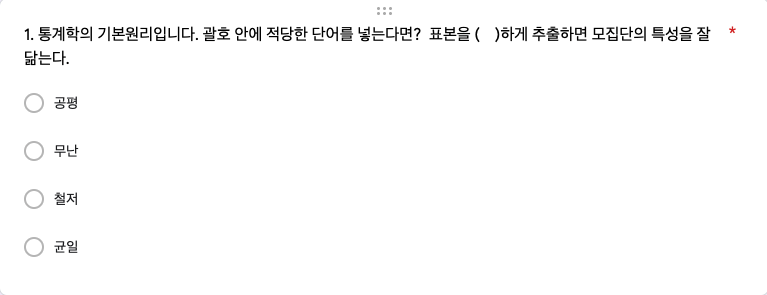
\includegraphics[width=0.75\linewidth]{./pics/Quiz210406_Q1} \end{flushleft}

\subsubsection{공평하게 추출하면
\ldots{}}\label{uxacf5uxd3c9uxd558uxac8c-uxcd94uxcd9cuxd558uxba74}

\begin{longtable}[]{@{}
  >{\raggedright\arraybackslash}p{(\columnwidth - 10\tabcolsep) * \real{0.1667}}
  >{\centering\arraybackslash}p{(\columnwidth - 10\tabcolsep) * \real{0.0972}}
  >{\centering\arraybackslash}p{(\columnwidth - 10\tabcolsep) * \real{0.0972}}
  >{\centering\arraybackslash}p{(\columnwidth - 10\tabcolsep) * \real{0.0972}}
  >{\centering\arraybackslash}p{(\columnwidth - 10\tabcolsep) * \real{0.0972}}
  >{\centering\arraybackslash}p{(\columnwidth - 10\tabcolsep) * \real{0.0972}}@{}}
\toprule\noalign{}
\begin{minipage}[b]{\linewidth}\raggedright
~
\end{minipage} & \begin{minipage}[b]{\linewidth}\centering
공평
\end{minipage} & \begin{minipage}[b]{\linewidth}\centering
무난
\end{minipage} & \begin{minipage}[b]{\linewidth}\centering
철저
\end{minipage} & \begin{minipage}[b]{\linewidth}\centering
균일
\end{minipage} & \begin{minipage}[b]{\linewidth}\centering
계
\end{minipage} \\
\midrule\noalign{}
\endhead
\bottomrule\noalign{}
\endlastfoot
\textbf{Red} & 62 & 2 & 1 & 21 & 86 \\
\textbf{Black} & 69 & 3 & 0 & 16 & 88 \\
\textbf{계} & 131 & 5 & 1 & 37 & 174 \\
\end{longtable}

\begin{longtable}[]{@{}
  >{\raggedleft\arraybackslash}p{(\columnwidth - 4\tabcolsep) * \real{0.2361}}
  >{\raggedleft\arraybackslash}p{(\columnwidth - 4\tabcolsep) * \real{0.0694}}
  >{\raggedleft\arraybackslash}p{(\columnwidth - 4\tabcolsep) * \real{0.1389}}@{}}
\caption{Pearson's Chi-squared test: \texttt{.}}\tabularnewline
\toprule\noalign{}
\begin{minipage}[b]{\linewidth}\raggedleft
Test statistic
\end{minipage} & \begin{minipage}[b]{\linewidth}\raggedleft
df
\end{minipage} & \begin{minipage}[b]{\linewidth}\raggedleft
P value
\end{minipage} \\
\midrule\noalign{}
\endfirsthead
\toprule\noalign{}
\begin{minipage}[b]{\linewidth}\raggedleft
Test statistic
\end{minipage} & \begin{minipage}[b]{\linewidth}\raggedleft
df
\end{minipage} & \begin{minipage}[b]{\linewidth}\raggedleft
P value
\end{minipage} \\
\midrule\noalign{}
\endhead
\bottomrule\noalign{}
\endlastfoot
2.227 & 3 & 0.5266 \\
\end{longtable}

Q1의 집계 결과가 Red, Black 간에 통계적으로 유의한 차이가 있는지
알아보기 위하여 카이제곱 테스트를 수행하였습니다.

그 결과 카이제곱 통계량은 2.23, 자유도는 3 , p-value 는 0.53이므로 Red,
Black 간에 통계적으로 유의한 차이를 보이지 않습니다.

실제로 닮은 게 느껴집니까?

\subsubsection{공평하게 추출하면 \ldots{}
(\%)}\label{uxacf5uxd3c9uxd558uxac8c-uxcd94uxcd9cuxd558uxba74-1}

\begin{longtable}[]{@{}
  >{\centering\arraybackslash}p{(\columnwidth - 8\tabcolsep) * \real{0.1111}}
  >{\centering\arraybackslash}p{(\columnwidth - 8\tabcolsep) * \real{0.0972}}
  >{\centering\arraybackslash}p{(\columnwidth - 8\tabcolsep) * \real{0.0972}}
  >{\centering\arraybackslash}p{(\columnwidth - 8\tabcolsep) * \real{0.1111}}
  >{\centering\arraybackslash}p{(\columnwidth - 8\tabcolsep) * \real{0.1250}}@{}}
\toprule\noalign{}
\begin{minipage}[b]{\linewidth}\centering
공평
\end{minipage} & \begin{minipage}[b]{\linewidth}\centering
무난
\end{minipage} & \begin{minipage}[b]{\linewidth}\centering
철저
\end{minipage} & \begin{minipage}[b]{\linewidth}\centering
균일
\end{minipage} & \begin{minipage}[b]{\linewidth}\centering
계
\end{minipage} \\
\midrule\noalign{}
\endhead
\bottomrule\noalign{}
\endlastfoot
75.29 & 2.87 & 0.57 & 21.26 & 100.00 \\
\end{longtable}

정답률은 Red, Black 을 합하여 계산하는데, 75.3(\%) 입니다.

\subsection{Q2. 리터러리 다이제스트의
실패}\label{q2.-uxb9acuxd130uxb7ecuxb9ac-uxb2e4uxc774uxc81cuxc2a4uxd2b8uxc758-uxc2e4uxd328}

\begin{flushleft}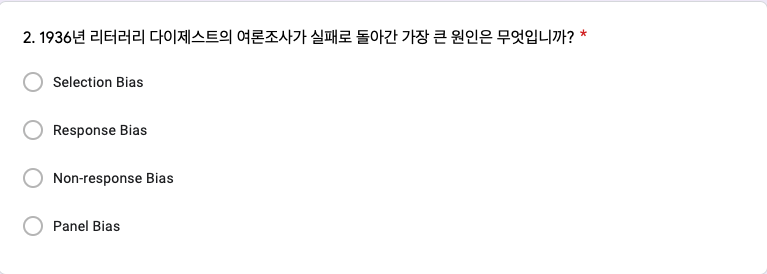
\includegraphics[width=0.75\linewidth]{./pics/Quiz210406_Q2} \end{flushleft}

\subsubsection{Selection Bias}\label{selection-bias}

\begin{longtable}[]{@{}
  >{\raggedright\arraybackslash}p{(\columnwidth - 10\tabcolsep) * \real{0.1429}}
  >{\raggedleft\arraybackslash}p{(\columnwidth - 10\tabcolsep) * \real{0.2024}}
  >{\raggedleft\arraybackslash}p{(\columnwidth - 10\tabcolsep) * \real{0.1905}}
  >{\raggedleft\arraybackslash}p{(\columnwidth - 10\tabcolsep) * \real{0.2381}}
  >{\raggedleft\arraybackslash}p{(\columnwidth - 10\tabcolsep) * \real{0.1548}}
  >{\centering\arraybackslash}p{(\columnwidth - 10\tabcolsep) * \real{0.0714}}@{}}
\toprule\noalign{}
\begin{minipage}[b]{\linewidth}\raggedright
~
\end{minipage} & \begin{minipage}[b]{\linewidth}\raggedleft
Selection Bias
\end{minipage} & \begin{minipage}[b]{\linewidth}\raggedleft
Response Bias
\end{minipage} & \begin{minipage}[b]{\linewidth}\raggedleft
Non-response Bias
\end{minipage} & \begin{minipage}[b]{\linewidth}\raggedleft
Panel Bias
\end{minipage} & \begin{minipage}[b]{\linewidth}\centering
계
\end{minipage} \\
\midrule\noalign{}
\endhead
\bottomrule\noalign{}
\endlastfoot
\textbf{Red} & 58 & 10 & 18 & 0 & 86 \\
\textbf{Black} & 60 & 7 & 16 & 5 & 88 \\
\textbf{계} & 118 & 17 & 34 & 5 & 174 \\
\end{longtable}

\begin{longtable}[]{@{}
  >{\raggedleft\arraybackslash}p{(\columnwidth - 4\tabcolsep) * \real{0.2361}}
  >{\raggedleft\arraybackslash}p{(\columnwidth - 4\tabcolsep) * \real{0.0694}}
  >{\raggedleft\arraybackslash}p{(\columnwidth - 4\tabcolsep) * \real{0.1389}}@{}}
\caption{Pearson's Chi-squared test: \texttt{.}}\tabularnewline
\toprule\noalign{}
\begin{minipage}[b]{\linewidth}\raggedleft
Test statistic
\end{minipage} & \begin{minipage}[b]{\linewidth}\raggedleft
df
\end{minipage} & \begin{minipage}[b]{\linewidth}\raggedleft
P value
\end{minipage} \\
\midrule\noalign{}
\endfirsthead
\toprule\noalign{}
\begin{minipage}[b]{\linewidth}\raggedleft
Test statistic
\end{minipage} & \begin{minipage}[b]{\linewidth}\raggedleft
df
\end{minipage} & \begin{minipage}[b]{\linewidth}\raggedleft
P value
\end{minipage} \\
\midrule\noalign{}
\endhead
\bottomrule\noalign{}
\endlastfoot
5.659 & 3 & 0.1294 \\
\end{longtable}

Q2의 집계 결과가 Red, Black 간에 통계적으로 유의한 차이가 있는지
알아보기 위하여 카이제곱 테스트를 수행하였습니다.

그 결과 카이제곱 통계량은 5.66, 자유도는 3, p-value 는 0.13이므로 Red,
Black 간에 통계적으로 유의한 차이를 보이지 않습니다.

실제로 닮은 게 느껴집니까?

\subsubsection{Selection Bias (\%)}\label{selection-bias-1}

\begin{longtable}[]{@{}
  >{\raggedleft\arraybackslash}p{(\columnwidth - 8\tabcolsep) * \real{0.2297}}
  >{\raggedleft\arraybackslash}p{(\columnwidth - 8\tabcolsep) * \real{0.2162}}
  >{\raggedleft\arraybackslash}p{(\columnwidth - 8\tabcolsep) * \real{0.2703}}
  >{\raggedleft\arraybackslash}p{(\columnwidth - 8\tabcolsep) * \real{0.1757}}
  >{\centering\arraybackslash}p{(\columnwidth - 8\tabcolsep) * \real{0.1081}}@{}}
\toprule\noalign{}
\begin{minipage}[b]{\linewidth}\raggedleft
Selection Bias
\end{minipage} & \begin{minipage}[b]{\linewidth}\raggedleft
Response Bias
\end{minipage} & \begin{minipage}[b]{\linewidth}\raggedleft
Non-response Bias
\end{minipage} & \begin{minipage}[b]{\linewidth}\raggedleft
Panel Bias
\end{minipage} & \begin{minipage}[b]{\linewidth}\centering
계
\end{minipage} \\
\midrule\noalign{}
\endhead
\bottomrule\noalign{}
\endlastfoot
67.8 & 9.8 & 19.5 & 2.9 & 100.0 \\
\end{longtable}

정답률은 Red, Black 을 합하여 계산하는데, 67.8(\%) 입니다.

\subsection{Q3. 1948년, 여론조사가 듀이를 당선시킨
해}\label{q3.-1948uxb144-uxc5ecuxb860uxc870uxc0acuxac00-uxb4c0uxc774uxb97c-uxb2f9uxc120uxc2dcuxd0a8-uxd574}

\begin{flushleft}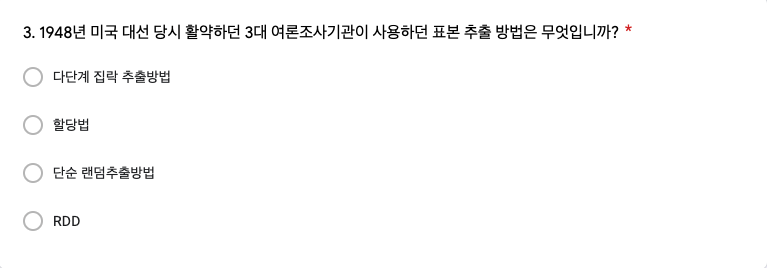
\includegraphics[width=0.75\linewidth]{./pics/Quiz210406_Q3} \end{flushleft}

\subsubsection{할당법의
문제점}\label{uxd560uxb2f9uxbc95uxc758-uxbb38uxc81cuxc810}

\begin{longtable}[]{@{}
  >{\raggedright\arraybackslash}p{(\columnwidth - 10\tabcolsep) * \real{0.1579}}
  >{\centering\arraybackslash}p{(\columnwidth - 10\tabcolsep) * \real{0.3026}}
  >{\centering\arraybackslash}p{(\columnwidth - 10\tabcolsep) * \real{0.1184}}
  >{\centering\arraybackslash}p{(\columnwidth - 10\tabcolsep) * \real{0.2632}}
  >{\raggedleft\arraybackslash}p{(\columnwidth - 10\tabcolsep) * \real{0.0789}}
  >{\centering\arraybackslash}p{(\columnwidth - 10\tabcolsep) * \real{0.0789}}@{}}
\toprule\noalign{}
\begin{minipage}[b]{\linewidth}\raggedright
~
\end{minipage} & \begin{minipage}[b]{\linewidth}\centering
다단계 집락 추출방법
\end{minipage} & \begin{minipage}[b]{\linewidth}\centering
할당법
\end{minipage} & \begin{minipage}[b]{\linewidth}\centering
단순 랜덤추출방법
\end{minipage} & \begin{minipage}[b]{\linewidth}\raggedleft
RDD
\end{minipage} & \begin{minipage}[b]{\linewidth}\centering
계
\end{minipage} \\
\midrule\noalign{}
\endhead
\bottomrule\noalign{}
\endlastfoot
\textbf{Red} & 7 & 61 & 13 & 5 & 86 \\
\textbf{Black} & 10 & 56 & 19 & 3 & 88 \\
\textbf{계} & 17 & 117 & 32 & 8 & 174 \\
\end{longtable}

\begin{longtable}[]{@{}
  >{\raggedleft\arraybackslash}p{(\columnwidth - 4\tabcolsep) * \real{0.2361}}
  >{\raggedleft\arraybackslash}p{(\columnwidth - 4\tabcolsep) * \real{0.0694}}
  >{\raggedleft\arraybackslash}p{(\columnwidth - 4\tabcolsep) * \real{0.1389}}@{}}
\caption{Pearson's Chi-squared test: \texttt{.}}\tabularnewline
\toprule\noalign{}
\begin{minipage}[b]{\linewidth}\raggedleft
Test statistic
\end{minipage} & \begin{minipage}[b]{\linewidth}\raggedleft
df
\end{minipage} & \begin{minipage}[b]{\linewidth}\raggedleft
P value
\end{minipage} \\
\midrule\noalign{}
\endfirsthead
\toprule\noalign{}
\begin{minipage}[b]{\linewidth}\raggedleft
Test statistic
\end{minipage} & \begin{minipage}[b]{\linewidth}\raggedleft
df
\end{minipage} & \begin{minipage}[b]{\linewidth}\raggedleft
P value
\end{minipage} \\
\midrule\noalign{}
\endhead
\bottomrule\noalign{}
\endlastfoot
2.345 & 3 & 0.5039 \\
\end{longtable}

Q3의 집계 결과가 Red, Black 간에 통계적으로 유의한 차이가 있는지
알아보기 위하여 카이제곱 테스트를 수행하였습니다.

그 결과 카이제곱 통계량은 2.35, 자유도는 3, p-value 는 0.50이므로 Red,
Black 간에 통계적으로 유의한 차이를 보이지 않습니다.

실제로 닮은 게 느껴집니까?

\subsubsection{할당법의
문제점(\%)}\label{uxd560uxb2f9uxbc95uxc758-uxbb38uxc81cuxc810-1}

\begin{longtable}[]{@{}
  >{\centering\arraybackslash}p{(\columnwidth - 8\tabcolsep) * \real{0.3194}}
  >{\centering\arraybackslash}p{(\columnwidth - 8\tabcolsep) * \real{0.1250}}
  >{\centering\arraybackslash}p{(\columnwidth - 8\tabcolsep) * \real{0.2778}}
  >{\raggedleft\arraybackslash}p{(\columnwidth - 8\tabcolsep) * \real{0.0833}}
  >{\centering\arraybackslash}p{(\columnwidth - 8\tabcolsep) * \real{0.1111}}@{}}
\toprule\noalign{}
\begin{minipage}[b]{\linewidth}\centering
다단계 집락 추출방법
\end{minipage} & \begin{minipage}[b]{\linewidth}\centering
할당법
\end{minipage} & \begin{minipage}[b]{\linewidth}\centering
단순 랜덤추출방법
\end{minipage} & \begin{minipage}[b]{\linewidth}\raggedleft
RDD
\end{minipage} & \begin{minipage}[b]{\linewidth}\centering
계
\end{minipage} \\
\midrule\noalign{}
\endhead
\bottomrule\noalign{}
\endlastfoot
9.8 & 67.2 & 18.4 & 4.6 & 100.0 \\
\end{longtable}

정답률은 Red, Black 을 합하여 계산하는데, 67.2(\%) 입니다.

\subsection{Q4. 1948 미 대선
이후}\label{q4.-1948-uxbbf8-uxb300uxc120-uxc774uxd6c4}

\begin{flushleft}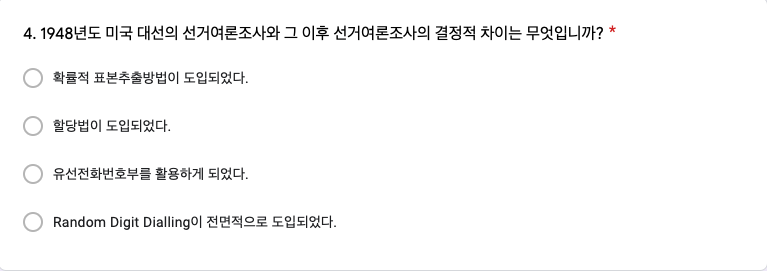
\includegraphics[width=0.75\linewidth]{./pics/Quiz210406_Q4} \end{flushleft}

\subsubsection{확률적 표본추출방법
도입}\label{uxd655uxb960uxc801-uxd45cuxbcf8uxcd94uxcd9cuxbc29uxbc95-uxb3c4uxc785}

\begin{longtable}[]{@{}
  >{\raggedright\arraybackslash}p{(\columnwidth - 10\tabcolsep) * \real{0.1667}}
  >{\centering\arraybackslash}p{(\columnwidth - 10\tabcolsep) * \real{0.2500}}
  >{\centering\arraybackslash}p{(\columnwidth - 10\tabcolsep) * \real{0.1250}}
  >{\centering\arraybackslash}p{(\columnwidth - 10\tabcolsep) * \real{0.2361}}
  >{\centering\arraybackslash}p{(\columnwidth - 10\tabcolsep) * \real{0.1389}}
  >{\centering\arraybackslash}p{(\columnwidth - 10\tabcolsep) * \real{0.0833}}@{}}
\toprule\noalign{}
\begin{minipage}[b]{\linewidth}\raggedright
~
\end{minipage} & \begin{minipage}[b]{\linewidth}\centering
확률적 표본추출
\end{minipage} & \begin{minipage}[b]{\linewidth}\centering
할당법
\end{minipage} & \begin{minipage}[b]{\linewidth}\centering
유선전화번호부
\end{minipage} & \begin{minipage}[b]{\linewidth}\centering
RDD도입
\end{minipage} & \begin{minipage}[b]{\linewidth}\centering
계
\end{minipage} \\
\midrule\noalign{}
\endhead
\bottomrule\noalign{}
\endlastfoot
\textbf{Red} & 62 & 10 & 8 & 6 & 86 \\
\textbf{Black} & 69 & 7 & 4 & 8 & 88 \\
\textbf{계} & 131 & 17 & 12 & 14 & 174 \\
\end{longtable}

\begin{longtable}[]{@{}
  >{\raggedleft\arraybackslash}p{(\columnwidth - 4\tabcolsep) * \real{0.2361}}
  >{\raggedleft\arraybackslash}p{(\columnwidth - 4\tabcolsep) * \real{0.0694}}
  >{\raggedleft\arraybackslash}p{(\columnwidth - 4\tabcolsep) * \real{0.1389}}@{}}
\caption{Pearson's Chi-squared test: \texttt{.}}\tabularnewline
\toprule\noalign{}
\begin{minipage}[b]{\linewidth}\raggedleft
Test statistic
\end{minipage} & \begin{minipage}[b]{\linewidth}\raggedleft
df
\end{minipage} & \begin{minipage}[b]{\linewidth}\raggedleft
P value
\end{minipage} \\
\midrule\noalign{}
\endfirsthead
\toprule\noalign{}
\begin{minipage}[b]{\linewidth}\raggedleft
Test statistic
\end{minipage} & \begin{minipage}[b]{\linewidth}\raggedleft
df
\end{minipage} & \begin{minipage}[b]{\linewidth}\raggedleft
P value
\end{minipage} \\
\midrule\noalign{}
\endhead
\bottomrule\noalign{}
\endlastfoot
2.5 & 3 & 0.4753 \\
\end{longtable}

Q4의 집계 결과가 Red, Black 간에 통계적으로 유의한 차이가 있는지
알아보기 위하여 카이제곱 테스트를 수행하였습니다.

그 결과 카이제곱 통계량은 2.50, 자유도는 3, p-value 는 0.48이므로 Red,
Black 간에 통계적으로 유의한 차이를 보이지 않습니다.

실제로 닮은 게 느껴집니까?

\subsubsection{확률적 표본추출방법 도입 \ldots{}
(\%)}\label{uxd655uxb960uxc801-uxd45cuxbcf8uxcd94uxcd9cuxbc29uxbc95-uxb3c4uxc785-1}

\begin{longtable}[]{@{}
  >{\centering\arraybackslash}p{(\columnwidth - 8\tabcolsep) * \real{0.2500}}
  >{\centering\arraybackslash}p{(\columnwidth - 8\tabcolsep) * \real{0.1250}}
  >{\centering\arraybackslash}p{(\columnwidth - 8\tabcolsep) * \real{0.2361}}
  >{\centering\arraybackslash}p{(\columnwidth - 8\tabcolsep) * \real{0.1389}}
  >{\centering\arraybackslash}p{(\columnwidth - 8\tabcolsep) * \real{0.1389}}@{}}
\toprule\noalign{}
\begin{minipage}[b]{\linewidth}\centering
확률적 표본추출
\end{minipage} & \begin{minipage}[b]{\linewidth}\centering
할당법
\end{minipage} & \begin{minipage}[b]{\linewidth}\centering
유선전화번호부
\end{minipage} & \begin{minipage}[b]{\linewidth}\centering
RDD도입
\end{minipage} & \begin{minipage}[b]{\linewidth}\centering
계
\end{minipage} \\
\midrule\noalign{}
\endhead
\bottomrule\noalign{}
\endlastfoot
75.3 & 9.8 & 6.9 & 8.0 & 100.0 \\
\end{longtable}

정답률은 Red, Black 을 합하여 계산하는데, 75.3(\%) 입니다.

\subsection{Q5. 표본오차를 반으로
줄이려면?}\label{q5.-uxd45cuxbcf8uxc624uxcc28uxb97c-uxbc18uxc73cuxb85c-uxc904uxc774uxb824uxba74}

\begin{flushleft}
\includegraphics[width=0.75\linewidth]{./pics/Quiz210406_Q5} \end{flushleft}

\subsubsection{4배로 늘려야}\label{uxbc30uxb85c-uxb298uxb824uxc57c}

\begin{longtable}[]{@{}
  >{\raggedright\arraybackslash}p{(\columnwidth - 10\tabcolsep) * \real{0.1667}}
  >{\centering\arraybackslash}p{(\columnwidth - 10\tabcolsep) * \real{0.1111}}
  >{\centering\arraybackslash}p{(\columnwidth - 10\tabcolsep) * \real{0.1111}}
  >{\centering\arraybackslash}p{(\columnwidth - 10\tabcolsep) * \real{0.1111}}
  >{\centering\arraybackslash}p{(\columnwidth - 10\tabcolsep) * \real{0.1111}}
  >{\centering\arraybackslash}p{(\columnwidth - 10\tabcolsep) * \real{0.1111}}@{}}
\toprule\noalign{}
\begin{minipage}[b]{\linewidth}\raggedright
~
\end{minipage} & \begin{minipage}[b]{\linewidth}\centering
2배로
\end{minipage} & \begin{minipage}[b]{\linewidth}\centering
4배로
\end{minipage} & \begin{minipage}[b]{\linewidth}\centering
1/2로
\end{minipage} & \begin{minipage}[b]{\linewidth}\centering
1/4로
\end{minipage} & \begin{minipage}[b]{\linewidth}\centering
계
\end{minipage} \\
\midrule\noalign{}
\endhead
\bottomrule\noalign{}
\endlastfoot
\textbf{Red} & 18 & 54 & 11 & 3 & 86 \\
\textbf{Black} & 24 & 53 & 10 & 1 & 88 \\
\textbf{계} & 42 & 107 & 21 & 4 & 174 \\
\end{longtable}

\begin{longtable}[]{@{}
  >{\raggedleft\arraybackslash}p{(\columnwidth - 4\tabcolsep) * \real{0.2361}}
  >{\raggedleft\arraybackslash}p{(\columnwidth - 4\tabcolsep) * \real{0.0694}}
  >{\raggedleft\arraybackslash}p{(\columnwidth - 4\tabcolsep) * \real{0.1389}}@{}}
\caption{Pearson's Chi-squared test: \texttt{.}}\tabularnewline
\toprule\noalign{}
\begin{minipage}[b]{\linewidth}\raggedleft
Test statistic
\end{minipage} & \begin{minipage}[b]{\linewidth}\raggedleft
df
\end{minipage} & \begin{minipage}[b]{\linewidth}\raggedleft
P value
\end{minipage} \\
\midrule\noalign{}
\endfirsthead
\toprule\noalign{}
\begin{minipage}[b]{\linewidth}\raggedleft
Test statistic
\end{minipage} & \begin{minipage}[b]{\linewidth}\raggedleft
df
\end{minipage} & \begin{minipage}[b]{\linewidth}\raggedleft
P value
\end{minipage} \\
\midrule\noalign{}
\endhead
\bottomrule\noalign{}
\endlastfoot
1.891 & 3 & 0.5953 \\
\end{longtable}

Q5의 집계 결과가 Red, Black 간에 통계적으로 유의한 차이가 있는지
알아보기 위하여 카이제곱 테스트를 수행하였습니다.

그 결과 카이제곱 통계량은 1.89, 자유도는 3, p-value 는 0.60이므로 Red,
Black 간에 통계적으로 유의한 차이를 보이지 않습니다.

실제로 닮은 게 느껴집니까?

\subsubsection{4배로 눌려야 (\%)}\label{uxbc30uxb85c-uxb20cuxb824uxc57c}

\begin{longtable}[]{@{}
  >{\centering\arraybackslash}p{(\columnwidth - 8\tabcolsep) * \real{0.1111}}
  >{\centering\arraybackslash}p{(\columnwidth - 8\tabcolsep) * \real{0.1111}}
  >{\centering\arraybackslash}p{(\columnwidth - 8\tabcolsep) * \real{0.1111}}
  >{\centering\arraybackslash}p{(\columnwidth - 8\tabcolsep) * \real{0.1111}}
  >{\centering\arraybackslash}p{(\columnwidth - 8\tabcolsep) * \real{0.1111}}@{}}
\toprule\noalign{}
\begin{minipage}[b]{\linewidth}\centering
2배로
\end{minipage} & \begin{minipage}[b]{\linewidth}\centering
4배로
\end{minipage} & \begin{minipage}[b]{\linewidth}\centering
1/2로
\end{minipage} & \begin{minipage}[b]{\linewidth}\centering
1/4로
\end{minipage} & \begin{minipage}[b]{\linewidth}\centering
계
\end{minipage} \\
\midrule\noalign{}
\endhead
\bottomrule\noalign{}
\endlastfoot
24.1 & 61.5 & 12.1 & 2.3 & 100.0 \\
\end{longtable}

정답률은 Red, Black 을 합하여 계산하는데, 61.5(\%) 입니다.

\subsection{Q6. 대선 여론조사의
목표모집단?}\label{q6.-uxb300uxc120-uxc5ecuxb860uxc870uxc0acuxc758-uxbaa9uxd45cuxbaa8uxc9d1uxb2e8}

\begin{flushleft}
\includegraphics[width=0.75\linewidth]{./pics/Quiz210406_Q6} \end{flushleft}

\subsubsection{선거당일 투표하는 유권자
전체}\label{uxc120uxac70uxb2f9uxc77c-uxd22cuxd45cuxd558uxb294-uxc720uxad8cuxc790-uxc804uxccb4}

\begin{longtable}[]{@{}
  >{\raggedright\arraybackslash}p{(\columnwidth - 10\tabcolsep) * \real{0.1132}}
  >{\centering\arraybackslash}p{(\columnwidth - 10\tabcolsep) * \real{0.1132}}
  >{\centering\arraybackslash}p{(\columnwidth - 10\tabcolsep) * \real{0.2075}}
  >{\centering\arraybackslash}p{(\columnwidth - 10\tabcolsep) * \real{0.1981}}
  >{\centering\arraybackslash}p{(\columnwidth - 10\tabcolsep) * \real{0.3113}}
  >{\centering\arraybackslash}p{(\columnwidth - 10\tabcolsep) * \real{0.0566}}@{}}
\toprule\noalign{}
\begin{minipage}[b]{\linewidth}\raggedright
~
\end{minipage} & \begin{minipage}[b]{\linewidth}\centering
국민 전체
\end{minipage} & \begin{minipage}[b]{\linewidth}\centering
18세 이상 국민 전체
\end{minipage} & \begin{minipage}[b]{\linewidth}\centering
등록된 유권자 전체
\end{minipage} & \begin{minipage}[b]{\linewidth}\centering
선거 당일 투표하는 유권자 전체
\end{minipage} & \begin{minipage}[b]{\linewidth}\centering
계
\end{minipage} \\
\midrule\noalign{}
\endhead
\bottomrule\noalign{}
\endlastfoot
\textbf{Red} & 6 & 18 & 14 & 48 & 86 \\
\textbf{Black} & 3 & 24 & 15 & 46 & 88 \\
\textbf{계} & 9 & 42 & 29 & 94 & 174 \\
\end{longtable}

\begin{longtable}[]{@{}
  >{\raggedleft\arraybackslash}p{(\columnwidth - 4\tabcolsep) * \real{0.2361}}
  >{\raggedleft\arraybackslash}p{(\columnwidth - 4\tabcolsep) * \real{0.0694}}
  >{\raggedleft\arraybackslash}p{(\columnwidth - 4\tabcolsep) * \real{0.1389}}@{}}
\caption{Pearson's Chi-squared test: \texttt{.}}\tabularnewline
\toprule\noalign{}
\begin{minipage}[b]{\linewidth}\raggedleft
Test statistic
\end{minipage} & \begin{minipage}[b]{\linewidth}\raggedleft
df
\end{minipage} & \begin{minipage}[b]{\linewidth}\raggedleft
P value
\end{minipage} \\
\midrule\noalign{}
\endfirsthead
\toprule\noalign{}
\begin{minipage}[b]{\linewidth}\raggedleft
Test statistic
\end{minipage} & \begin{minipage}[b]{\linewidth}\raggedleft
df
\end{minipage} & \begin{minipage}[b]{\linewidth}\raggedleft
P value
\end{minipage} \\
\midrule\noalign{}
\endhead
\bottomrule\noalign{}
\endlastfoot
1.911 & 3 & 0.591 \\
\end{longtable}

Q6의 집계 결과가 Red, Black 간에 통계적으로 유의한 차이가 있는지
알아보기 위하여 카이제곱 테스트를 수행하였습니다.

그 결과 카이제곱 통계량은 1.91, 자유도는 3, p-value 는 0.59이므로 Red,
Black 간에 통계적으로 유의한 차이를 보이지 않습니다.

실제로 닮은 게 느껴집니까?

\subsubsection{선거당일 투표하는 유권자
전체(\%)}\label{uxc120uxac70uxb2f9uxc77c-uxd22cuxd45cuxd558uxb294-uxc720uxad8cuxc790-uxc804uxccb4-1}

\begin{longtable}[]{@{}
  >{\centering\arraybackslash}p{(\columnwidth - 8\tabcolsep) * \real{0.1250}}
  >{\centering\arraybackslash}p{(\columnwidth - 8\tabcolsep) * \real{0.2292}}
  >{\centering\arraybackslash}p{(\columnwidth - 8\tabcolsep) * \real{0.2188}}
  >{\centering\arraybackslash}p{(\columnwidth - 8\tabcolsep) * \real{0.3438}}
  >{\centering\arraybackslash}p{(\columnwidth - 8\tabcolsep) * \real{0.0833}}@{}}
\toprule\noalign{}
\begin{minipage}[b]{\linewidth}\centering
국민 전체
\end{minipage} & \begin{minipage}[b]{\linewidth}\centering
18세 이상 국민 전체
\end{minipage} & \begin{minipage}[b]{\linewidth}\centering
등록된 유권자 전체
\end{minipage} & \begin{minipage}[b]{\linewidth}\centering
선거 당일 투표하는 유권자 전체
\end{minipage} & \begin{minipage}[b]{\linewidth}\centering
계
\end{minipage} \\
\midrule\noalign{}
\endhead
\bottomrule\noalign{}
\endlastfoot
5.2 & 24.1 & 16.7 & 54.0 & 100.0 \\
\end{longtable}

정답률은 Red, Black 을 합하여 계산하는데, 54.0(\%) 입니다.

\subsection{Wason Selection Task}\label{wason-selection-task}

같은 구조의 문제를 추상적으로 물어볼 때와 구체적으로 사례를 들어서
물어볼 때의 정답률에 큰 차이가 있음에 유의하세요.

Red 집단에게는 추상적 질문을 먼저 던지고, 구체적 사례를 든 질문을 나중에
던졌으며 Black 집단에게는 구체적 사례를 든 질문을 먼저 던지고, 추상적
질문을 나중에 던졌습니다.

추상적인 질문에 대해서는 매우 낮은 정답률을 보이지만 구체적인 질문에
대해서는 정답률이 훨씬 올라가는 것을 관찰할 수 있습니다.

추상적인 질문에 쩔쩔매는 것이 정상입니다.

Wason Selection Task 는 인지 편향, 그 중에서도 확증 편향이 많은
사람들에게 공통적으로 나타난다는 것을 보여줍니다.

반증의 근거가 되는 자료는 잘 들여다 보려 하지 않습니다.

이 실험 결과의 어느 부분이 이를 입증하는 지 살펴 봅니다.

\subsubsection{Red. Q7에 추상적 문제, Q8에 구체적
문제}\label{red.-q7uxc5d0-uxcd94uxc0c1uxc801-uxbb38uxc81c-q8uxc5d0-uxad6cuxccb4uxc801-uxbb38uxc81c}

\begin{flushleft}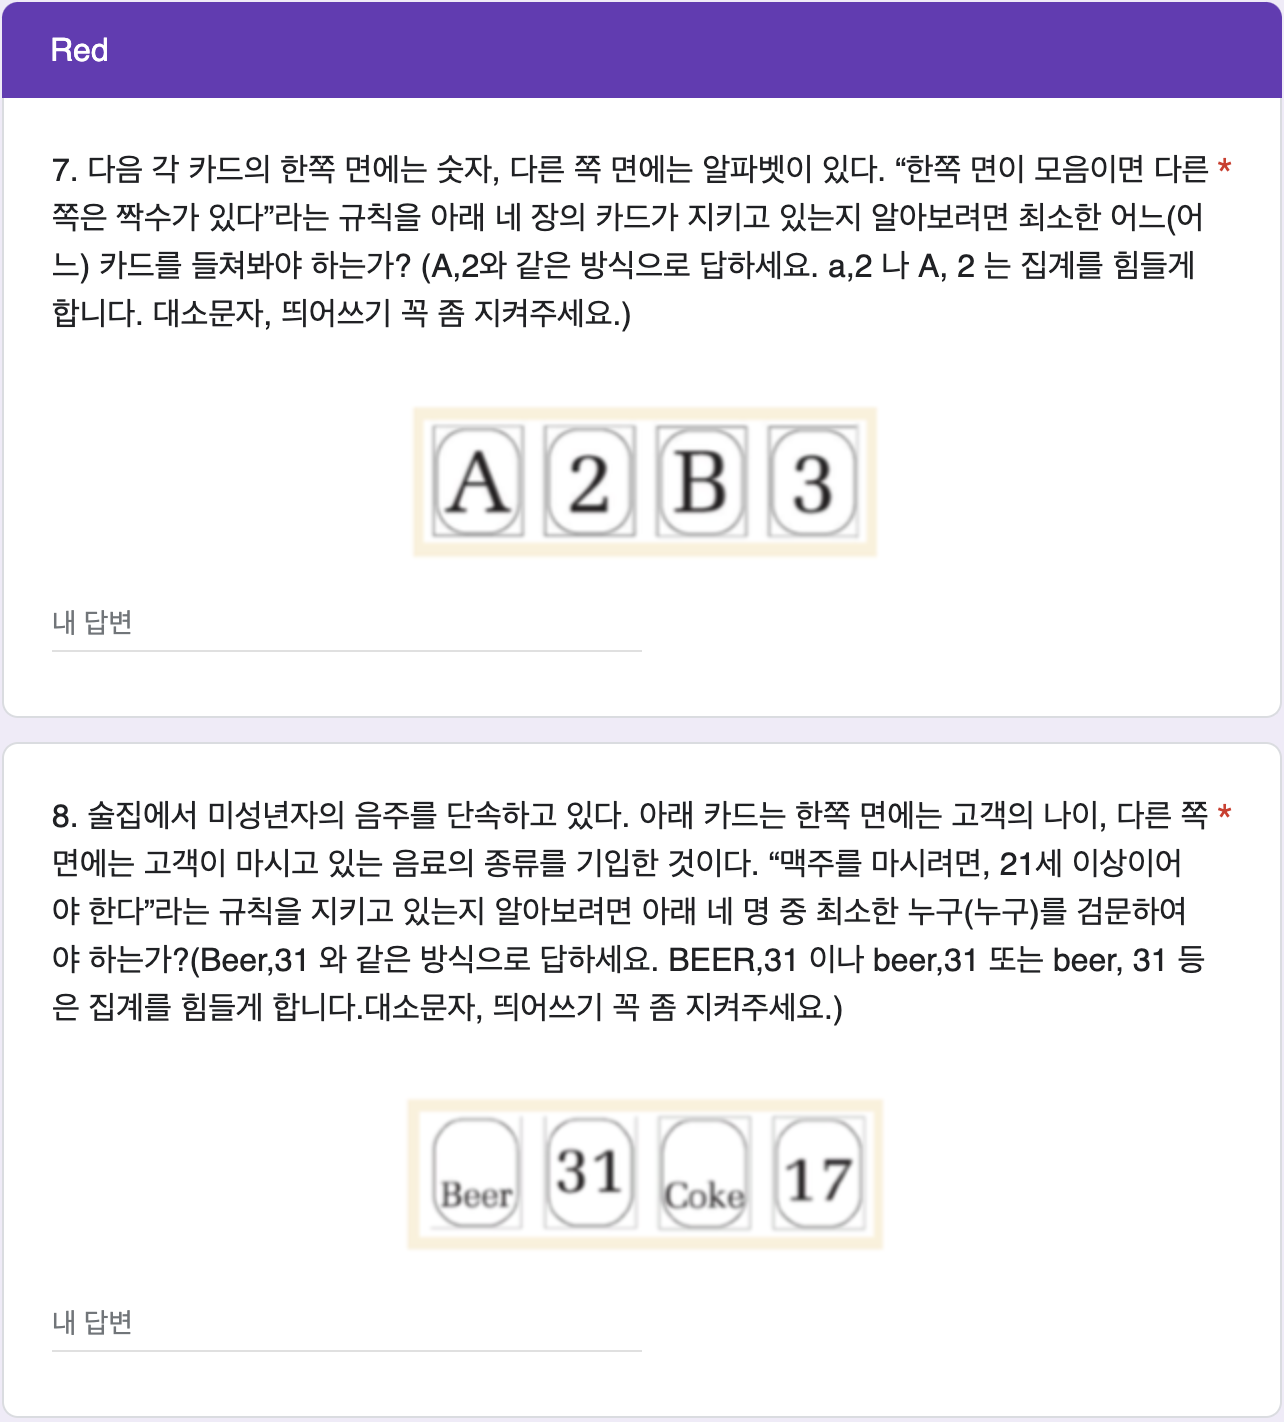
\includegraphics[width=0.75\linewidth]{./pics/Quiz240412_Q7_Red} \end{flushleft}

\subsubsection{Black. Q7에 구체적 문제, Q8에 추상적
문제}\label{black.-q7uxc5d0-uxad6cuxccb4uxc801-uxbb38uxc81c-q8uxc5d0-uxcd94uxc0c1uxc801-uxbb38uxc81c}

\begin{flushleft}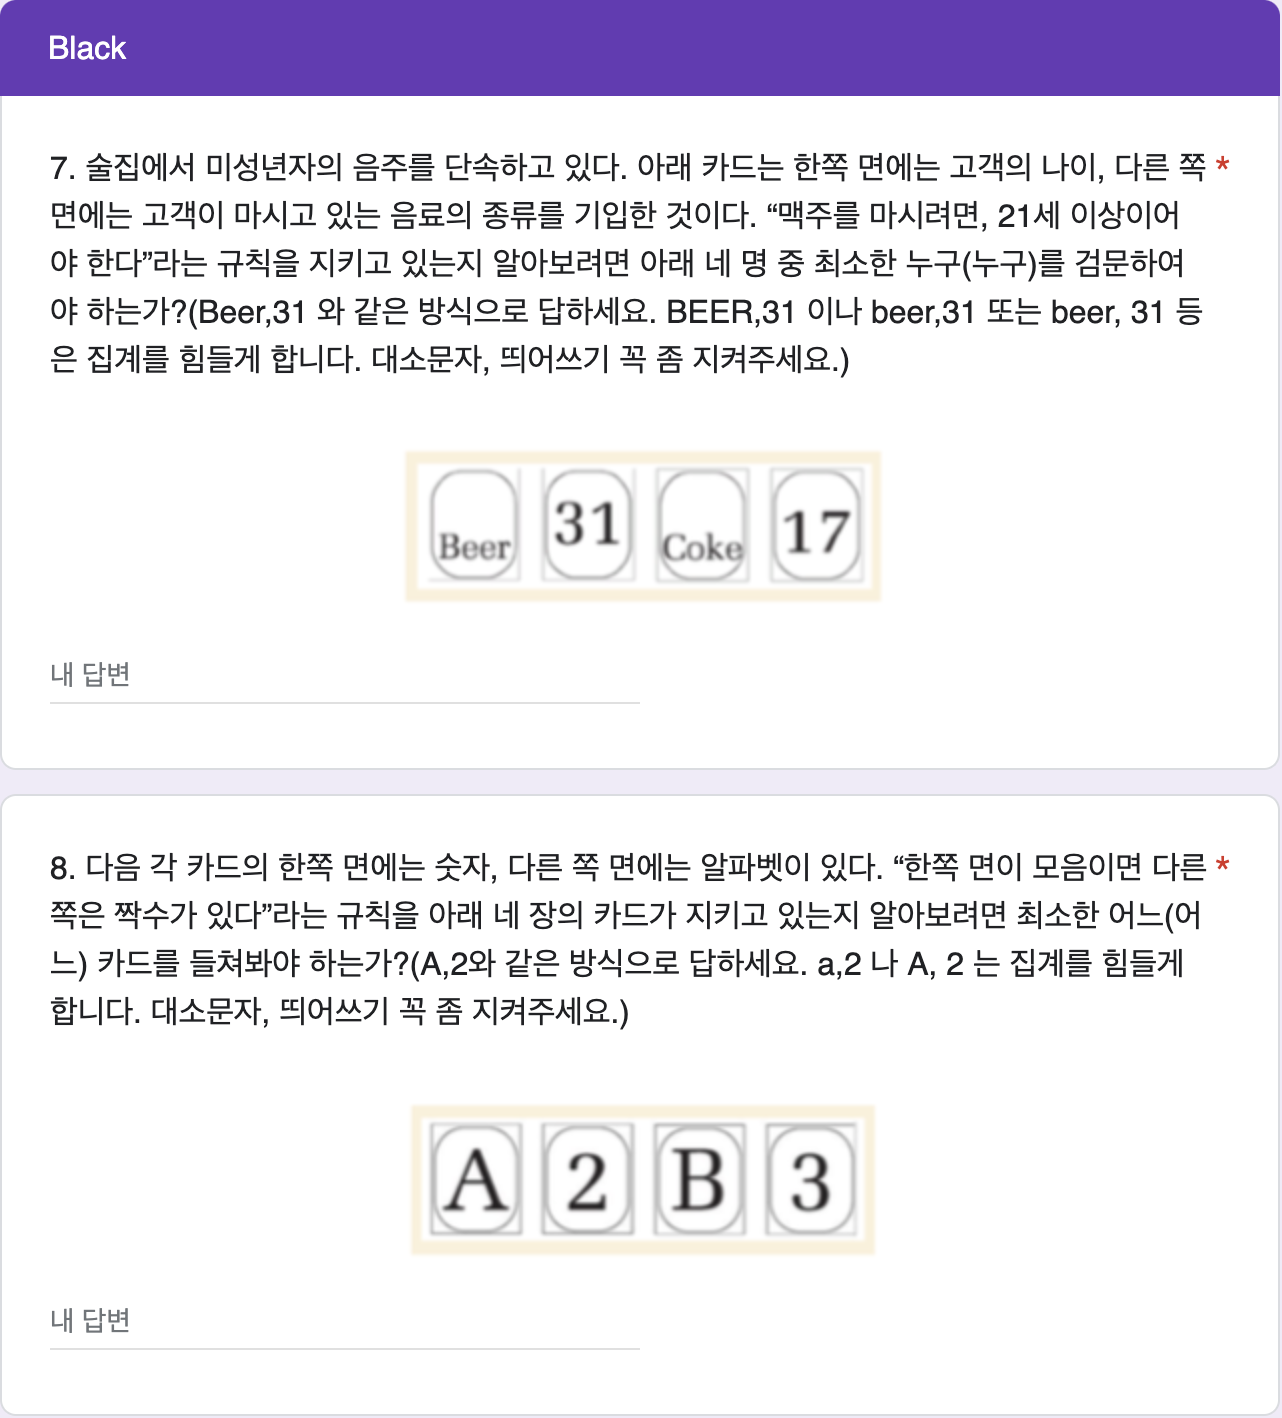
\includegraphics[width=0.75\linewidth]{./pics/Quiz240412_Q7_Black} \end{flushleft}

\subsection{Q7. Red에 추상적 질문, Black에 구체적
질문}\label{q7.-reduxc5d0-uxcd94uxc0c1uxc801-uxc9c8uxbb38-blackuxc5d0-uxad6cuxccb4uxc801-uxc9c8uxbb38}

``한쪽 면이 모음이면 다른 쪽은 짝수가 있다.''

이 규칙은 ``X이면 Y이다''의 형식으로 되어 있습니다.

이 논리식과 동등한 것은 \textbf{대우}인 ``Y가 아니면 X가 아니다''입니다.

매우 불편한 구조이죠.

그렇다 보니까 이게 잘 떠오를 리가 없습니다.

'선거여론조사의 발달'에서 학습한 바 있는 ``표본을 공평하게 뽑으면
모집단의 특성을 잘 닮는다''의 대우가 바로 ``모집단을 닮지 않으면 표본을
공평하게 뽑지 않은 것이다''입니다.

즉, 표본을 공평하게 뽑지 않아서 모집단을 제대로 닮지 않은 표본을
뽑았다는 것이죠.

주어진 네 장의 카드 중에서 한쪽 면이 모음인 것은 A입니다.

따라서 A는 우선 들쳐봐야 하는 카드이고, ``한쪽 면이 모음이면 다른 쪽은
짝수가 있다''의 대우는 ``한쪽 면이 짝수가 아니면 다른 쪽 면이 모음이
아니다'', 즉 ``한쪽 면이 홀수이면 다른 쪽 면은 자음이다''가 됩니다.

짝수가 아니면 홀수이고, 모음이 아니면 자음이니까요.

따라서 홀수 카드를 들쳐봐야 합니다.

그래서 A,3 두 장을 들쳐보면 됩니다.

맥주와 연령 문제는 실생활과 밀접한 구체적인 사안이어서 ``어, 맥주 마시는
사람 신분증 좀 보여주세요, 17살 미성년자는 지금 마시는 것이
맥주인가요?''하고 묻는 데 익숙하지만 직관적으로 Beer와 17을 검문해야
한다고 추론하였는지 논증하는 연습이 필요합니다.

``맥주를 마시려면, 21세 이상이어야 한다''라는 규칙으로부터 ``맥주''를
검문해야 하고, 검문으로부터 나이를 확인합니다.

그리고 이 규칙과 동등한 대우인 ``21세 이상이 아니면, 맥주를 마실 수
없다'', 즉, ``21세 미만이면 맥주를 마실 수 없다''로부터 ``21세 미만''인
``17세''를 검문해야 하는 것입니다.

물론 실생활에서 접할 수 있는 문제이기 때문에 미성년자가 맥주를 마시고
있는 것은 아닌지 Beer와 17을 골라야 한다고 쉽게 답할 수 있지만 그
배경에는 이러한 논리가 숨어 있습니다.

\subsubsection{집계}\label{uxc9d1uxacc4}

\begin{longtable}[]{@{}
  >{\raggedright\arraybackslash}p{(\columnwidth - 6\tabcolsep) * \real{0.3472}}
  >{\centering\arraybackslash}p{(\columnwidth - 6\tabcolsep) * \real{0.0972}}
  >{\centering\arraybackslash}p{(\columnwidth - 6\tabcolsep) * \real{0.0972}}
  >{\centering\arraybackslash}p{(\columnwidth - 6\tabcolsep) * \real{0.0972}}@{}}
\caption{Red에 추상적 질문, Black에 구체적 질문}\tabularnewline
\toprule\noalign{}
\begin{minipage}[b]{\linewidth}\raggedright
~
\end{minipage} & \begin{minipage}[b]{\linewidth}\centering
정답
\end{minipage} & \begin{minipage}[b]{\linewidth}\centering
오답
\end{minipage} & \begin{minipage}[b]{\linewidth}\centering
계
\end{minipage} \\
\midrule\noalign{}
\endfirsthead
\toprule\noalign{}
\begin{minipage}[b]{\linewidth}\raggedright
~
\end{minipage} & \begin{minipage}[b]{\linewidth}\centering
정답
\end{minipage} & \begin{minipage}[b]{\linewidth}\centering
오답
\end{minipage} & \begin{minipage}[b]{\linewidth}\centering
계
\end{minipage} \\
\midrule\noalign{}
\endhead
\bottomrule\noalign{}
\endlastfoot
\textbf{Red(추상적 질문)} & 29 & 57 & 86 \\
\textbf{Black(구체적 질문)} & 52 & 36 & 88 \\
\textbf{계} & 81 & 93 & 174 \\
\end{longtable}

\{A, 2, B, 3\}에서 어느 카드를(들을) 골라야 ``한쪽 면이 모음이면, 다른
쪽 면은 짝수이다''라는 규칙을 지키고 있는 지 확인할 수 있는가? 라는
질문을 Red에 배치하고, \{Beer, 31, Coke, 17\}에서 누구를(들을) 검문해야
하는가라는 질문을 Black에 배치했습니다.

Red의 경우 총 86(명)이 응답하였고 29(명)이 정답인 \{A, 3\}를 올렸습니다.

구체적인 상황에 놓인 Black의 경우 총 88(명)이 응답하였고 52(명)이 정답인
\{Beer,17\}을 올려서 구체적인 질문에 압도적으로 많은 정답이 나온 것을 알
수 있습니다.

이를 백분율로 비교해 보면

\subsubsection{\% 비교}\label{uxbe44uxad50}

\begin{longtable}[]{@{}
  >{\raggedright\arraybackslash}p{(\columnwidth - 6\tabcolsep) * \real{0.3472}}
  >{\centering\arraybackslash}p{(\columnwidth - 6\tabcolsep) * \real{0.0972}}
  >{\centering\arraybackslash}p{(\columnwidth - 6\tabcolsep) * \real{0.0972}}
  >{\centering\arraybackslash}p{(\columnwidth - 6\tabcolsep) * \real{0.1111}}@{}}
\toprule\noalign{}
\begin{minipage}[b]{\linewidth}\raggedright
~
\end{minipage} & \begin{minipage}[b]{\linewidth}\centering
정답
\end{minipage} & \begin{minipage}[b]{\linewidth}\centering
오답
\end{minipage} & \begin{minipage}[b]{\linewidth}\centering
계
\end{minipage} \\
\midrule\noalign{}
\endhead
\bottomrule\noalign{}
\endlastfoot
\textbf{Red(추상적 질문)} & 33.7 & 66.3 & 100.0 \\
\textbf{Black(구체적 질문)} & 59.1 & 40.9 & 100.0 \\
\end{longtable}

추상적인 질문으로 이루어진 Red에서는 33.7(\%)가 정답을 올렸고, 구체적인
질문으로 이루어진 Black에서는 59.1(\%)가 정답을 올려서 구체적인 질문에
압도적으로 많은 정답이 올라왔다는 것을 알 수 있습니다.

이 상황을 Mosiac Plot으로 살펴보겠습니다.

\subsubsection{Mosaic Plot}\label{mosaic-plot}

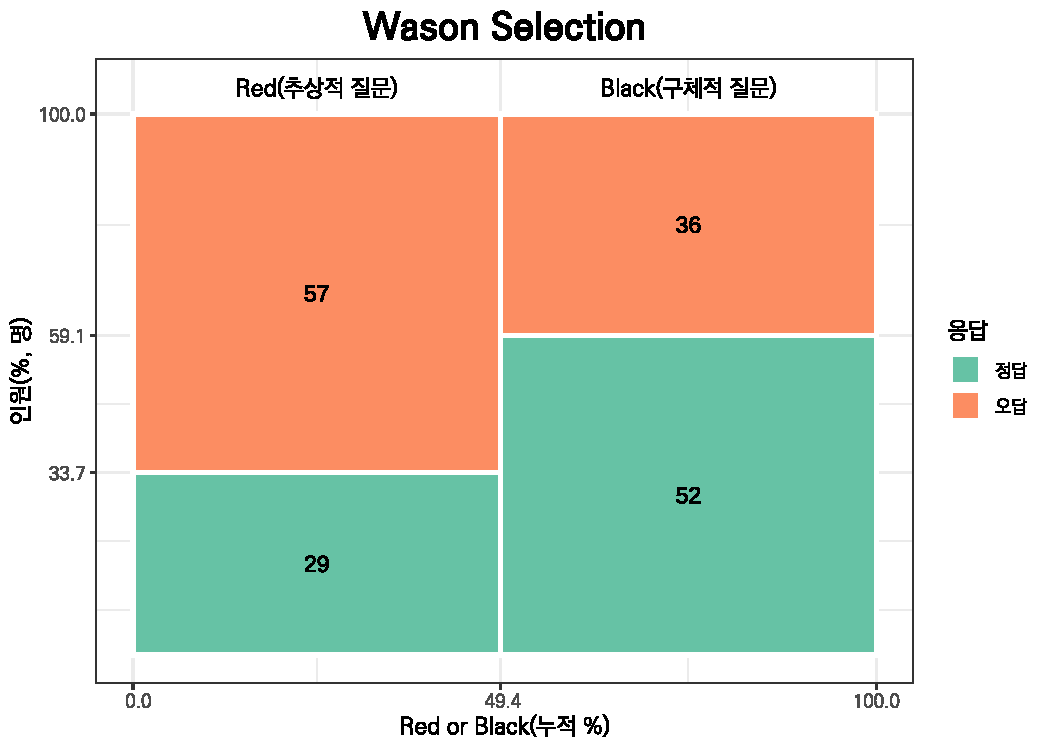
\includegraphics{quiz250414_Report_v4_files/figure-latex/mosaic plot1-1.pdf}

Mosaic Plot으로부터 추상적 질문이 주어진 Red 에서 정답 비율이 구체적
질문이 주어진 Black 에서 정답 비율에 비해서 매우 적다는 것을 시각적으로
파악할 수 있습니다.

\subsection{Q8. Red에 구체적 질문, Black에 추상적
질문}\label{q8.-reduxc5d0-uxad6cuxccb4uxc801-uxc9c8uxbb38-blackuxc5d0-uxcd94uxc0c1uxc801-uxc9c8uxbb38}

Q8에서는 Q7과 반대로 Red에 구체적 질문, Black에 추상적 질문을
배치하였습니다.

이렇게 하므로써 질문지에 응답한 모든 사람은 한 번씩 구체적 질문과 추상적
질문에 답할 수 있게 되었습니다.

집계 결과는 비슷합니다.

다만, 이렇게 추상적 질문을 먼저 배치하고 구체적 질문을 나중에
배치하느냐, 혹은 그 반대로 구체적 질문을 먼저 배치하고 추상적 질문을
나중에 배치한 것의 영향이 있는지를 파악한다면 학습 순서가 정답률과 어떤
관계가 있는지 파악할 수 있지 않을까 합니다.

\subsubsection{집계}\label{uxc9d1uxacc4-1}

\begin{longtable}[]{@{}
  >{\raggedright\arraybackslash}p{(\columnwidth - 6\tabcolsep) * \real{0.3472}}
  >{\centering\arraybackslash}p{(\columnwidth - 6\tabcolsep) * \real{0.0972}}
  >{\centering\arraybackslash}p{(\columnwidth - 6\tabcolsep) * \real{0.0972}}
  >{\centering\arraybackslash}p{(\columnwidth - 6\tabcolsep) * \real{0.0972}}@{}}
\caption{Red에 구체적 질문, Black에 추상적 질문}\tabularnewline
\toprule\noalign{}
\begin{minipage}[b]{\linewidth}\raggedright
~
\end{minipage} & \begin{minipage}[b]{\linewidth}\centering
정답
\end{minipage} & \begin{minipage}[b]{\linewidth}\centering
오답
\end{minipage} & \begin{minipage}[b]{\linewidth}\centering
계
\end{minipage} \\
\midrule\noalign{}
\endfirsthead
\toprule\noalign{}
\begin{minipage}[b]{\linewidth}\raggedright
~
\end{minipage} & \begin{minipage}[b]{\linewidth}\centering
정답
\end{minipage} & \begin{minipage}[b]{\linewidth}\centering
오답
\end{minipage} & \begin{minipage}[b]{\linewidth}\centering
계
\end{minipage} \\
\midrule\noalign{}
\endhead
\bottomrule\noalign{}
\endlastfoot
\textbf{Red(구체적 질문)} & 55 & 31 & 86 \\
\textbf{Black(추상적 질문)} & 25 & 63 & 88 \\
\textbf{계} & 80 & 94 & 174 \\
\end{longtable}

구체적인 질문을 배치한 Red의 경우 총 86(명)이 응답하였고 55(명)이 정답인
\{Beer, 17\}(을)를 올렸습니다.

추상적인 질문을 배치한 Black의 경우 총 88(명)이 응답하였고 25(명)이
정답인 \{A,3\}(을)를 올려서 구체적인 질문에 압도적으로 많은 정답이 나온
것을 알 수 있습니다.

이를 백분율로 비교해 보면

\subsubsection{\% 비교.}\label{uxbe44uxad50.}

\begin{longtable}[]{@{}
  >{\raggedright\arraybackslash}p{(\columnwidth - 6\tabcolsep) * \real{0.3472}}
  >{\centering\arraybackslash}p{(\columnwidth - 6\tabcolsep) * \real{0.0972}}
  >{\centering\arraybackslash}p{(\columnwidth - 6\tabcolsep) * \real{0.0972}}
  >{\centering\arraybackslash}p{(\columnwidth - 6\tabcolsep) * \real{0.1111}}@{}}
\toprule\noalign{}
\begin{minipage}[b]{\linewidth}\raggedright
~
\end{minipage} & \begin{minipage}[b]{\linewidth}\centering
정답
\end{minipage} & \begin{minipage}[b]{\linewidth}\centering
오답
\end{minipage} & \begin{minipage}[b]{\linewidth}\centering
계
\end{minipage} \\
\midrule\noalign{}
\endhead
\bottomrule\noalign{}
\endlastfoot
\textbf{Red(구체적 질문)} & 64.0 & 36.0 & 100.0 \\
\textbf{Black(추상적 질문)} & 28.4 & 71.6 & 100.0 \\
\end{longtable}

구체적인 질문을 배치한 Red에서는 64.0(\%)가 정답을 올렸고, 추상적인
질문을 배치한 Black에서는 28.4(\%)가 정답을 올려서 구체적인 질문에
압도적으로 많은 정답이 올라왔다는 것을 알 수 있습니다.

이 상황을 Mosaic Plot으로 살펴보겠습니다.

\subsubsection{Mosaic Plot}\label{mosaic-plot-1}

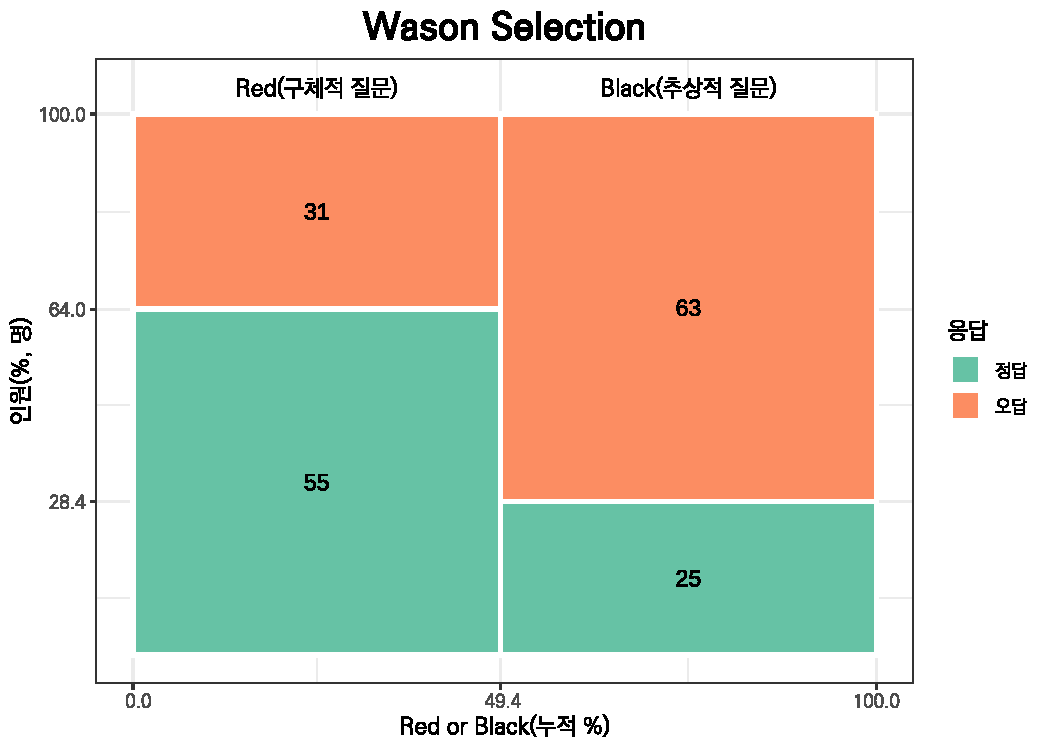
\includegraphics{quiz250414_Report_v4_files/figure-latex/mosaic plot2-1.pdf}

Mosaic Plot으로부터 구체적 질문이 주어진 Red 의 정답 비율이 추상적
질문이 주어진 Black의 정답 비율에 비해서 매우 높다는 것을 시각적으로
파악할 수 있습니다.

\subsection{Q9. 인지적 편향과
오류}\label{q9.-uxc778uxc9c0uxc801-uxd3b8uxd5a5uxacfc-uxc624uxb958}

Wason Selection Task 에서 많은 사람들이 겪는 흔한 오류(예 : 확증편향)을
설명합니다.

사람들은 보통 자신의 가설을 확인하기 위한 정보만 찾고, 반례가 될 수 있는
카드는 무시하려는 경향이 있습니다.

Peter C. Wason (1924-2003)의 연구에 의하면 정답을 찾아내는 백분율은
10\%에 불과합니다.

여러분의 응답과 비교해 보세요.

\subsubsection{집계}\label{uxc9d1uxacc4-2}

\begin{longtable}[]{@{}
  >{\raggedright\arraybackslash}p{(\columnwidth - 8\tabcolsep) * \real{0.4167}}
  >{\raggedleft\arraybackslash}p{(\columnwidth - 8\tabcolsep) * \real{0.0833}}
  >{\raggedleft\arraybackslash}p{(\columnwidth - 8\tabcolsep) * \real{0.0833}}
  >{\raggedleft\arraybackslash}p{(\columnwidth - 8\tabcolsep) * \real{0.1111}}
  >{\centering\arraybackslash}p{(\columnwidth - 8\tabcolsep) * \real{0.1111}}@{}}
\caption{Wason Selection Task 인지편향 분석}\tabularnewline
\toprule\noalign{}
\begin{minipage}[b]{\linewidth}\raggedright
~
\end{minipage} & \begin{minipage}[b]{\linewidth}\raggedleft
A,2
\end{minipage} & \begin{minipage}[b]{\linewidth}\raggedleft
A,3
\end{minipage} & \begin{minipage}[b]{\linewidth}\raggedleft
Other
\end{minipage} & \begin{minipage}[b]{\linewidth}\centering
계
\end{minipage} \\
\midrule\noalign{}
\endfirsthead
\toprule\noalign{}
\begin{minipage}[b]{\linewidth}\raggedright
~
\end{minipage} & \begin{minipage}[b]{\linewidth}\raggedleft
A,2
\end{minipage} & \begin{minipage}[b]{\linewidth}\raggedleft
A,3
\end{minipage} & \begin{minipage}[b]{\linewidth}\raggedleft
Other
\end{minipage} & \begin{minipage}[b]{\linewidth}\centering
계
\end{minipage} \\
\midrule\noalign{}
\endhead
\bottomrule\noalign{}
\endlastfoot
\textbf{Red(추상적 질문 먼저)} & 34 & 27 & 25 & 86 \\
\textbf{Black(구체적 질문 먼저)} & 45 & 22 & 21 & 88 \\
\textbf{계} & 79 & 49 & 46 & 174 \\
\end{longtable}

\{A, 2, B, 3\}에서 어느 카드를(들을) 골라야 ``한쪽 면이 모음이면, 다른
쪽 면은 짝수이다''라는 규칙을 지키고 있는 지 확인할 수 있는가? 라는
질문이 Q7에 먼저 나오는 것을 Red에 배치하고, Black 에서는 \{A, 2, B,
3\}에 대한 질문이 Q8에 나오도록 배치했습니다.

많은 사람들은 이 질문에 대해서 A와 2를 뒤집으려 합니다.

A는 모음이니까 확인해야 할 것 같고, 2는 짝수이니까 확인하려고 듭니다.

여기서 확증 편향이 나타납니다.

사람들은 주어진 규칙을 확인하기 위해 당장 눈에 들어오는 모음과 짝수, 즉
A와 2를 확인하려는 경향이 강합니다.

그러나 논리적으로 규칙을 검증하려면 짝수가 아닌 홀수 카드를 뒤집어야
합니다.

``한쪽 면이 모음이면, 다른 쪽 면은 짝수이다''와 동등한 규칙은 ``한쪽
면이 짝수가 아니면, 다른 쪽 면은 모응이 아니다''이기 때문입니다.

짝수가 아니면 홀수이니까 3을 뒤집어야 하는 것이죠.

추상적 질문이 먼저 Q7에 나온 Red의 경우 총 86(명)이 응답하였고 34(명)이
확증편향에서 비롯된 \{A,2\}를 올렸습니다.

정답인 \{A,3\}를 올린 27(명)보다 훨씬 많습니다.

추상적 질문이 Q8에 나온 Black 의 경우 총 88(명)이 응답하였고 45(명)이
확증편향에서 비롯된 \{A,2\}를 올렸습니다.

정답인 \{A,3\}를 올린 22(명)보다 훨씬 많습니다.

합해서 79(명)이 확증편향에서 비롯된 \{A,2\}를 올렸고, 49(명)이 정답인
\{A,3\}를 올렸습니다.

이는 확증편향에서 비롯된 응답이 정답의 2배를 넘을 정도로 많다는 것을
보여줍니다.

백분율로 살펴 보겠습니다.

\subsubsection{\% 비교.}\label{uxbe44uxad50.-1}

\begin{longtable}[]{@{}
  >{\raggedright\arraybackslash}p{(\columnwidth - 8\tabcolsep) * \real{0.4167}}
  >{\raggedleft\arraybackslash}p{(\columnwidth - 8\tabcolsep) * \real{0.0972}}
  >{\raggedleft\arraybackslash}p{(\columnwidth - 8\tabcolsep) * \real{0.0972}}
  >{\raggedleft\arraybackslash}p{(\columnwidth - 8\tabcolsep) * \real{0.1111}}
  >{\centering\arraybackslash}p{(\columnwidth - 8\tabcolsep) * \real{0.1111}}@{}}
\toprule\noalign{}
\begin{minipage}[b]{\linewidth}\raggedright
~
\end{minipage} & \begin{minipage}[b]{\linewidth}\raggedleft
A,2
\end{minipage} & \begin{minipage}[b]{\linewidth}\raggedleft
A,3
\end{minipage} & \begin{minipage}[b]{\linewidth}\raggedleft
Other
\end{minipage} & \begin{minipage}[b]{\linewidth}\centering
계
\end{minipage} \\
\midrule\noalign{}
\endhead
\bottomrule\noalign{}
\endlastfoot
\textbf{Red(추상적 질문 먼저)} & 39.5 & 31.4 & 29.1 & 100.0 \\
\textbf{Black(구체적 질문 먼저)} & 51.1 & 25.0 & 23.9 & 100.0 \\
\textbf{계} & 45.4 & 28.2 & 26.4 & 100.0 \\
\end{longtable}

추상적인 질문이 먼저 Q7에 나온 Red에서는 39.5(\%)가 확증편향에서 비롯된
응답 \{A,2\}를 올렸고, 31.4(\%)가 정답인 \{A,3\}을 올렸는데, 추상적인
질문이 나중에 Q8에 나온 Black 에서는 51.1(\%)가 확증편향에서 비롯된 응답
\{A,2\}를 올렸고, 25.0(\%)가 정답인 \{A,3\}을 올렸습니다.

합해서 보면 45.4(\%)가 확증편향에서 비롯된 응답 \{A,2\}를 올렸고,
28.2(\%)가 정답인 \{A,3\}을 올렸습니다.

확증편향으로 인한 응답이 정답보다 2배를 넘어가는 것을 다시 확인할 수
있습니다.

이 상황을 Mosiac Plot으로 살펴보겠습니다.

\subsubsection{Mosaic Plot}\label{mosaic-plot-2}

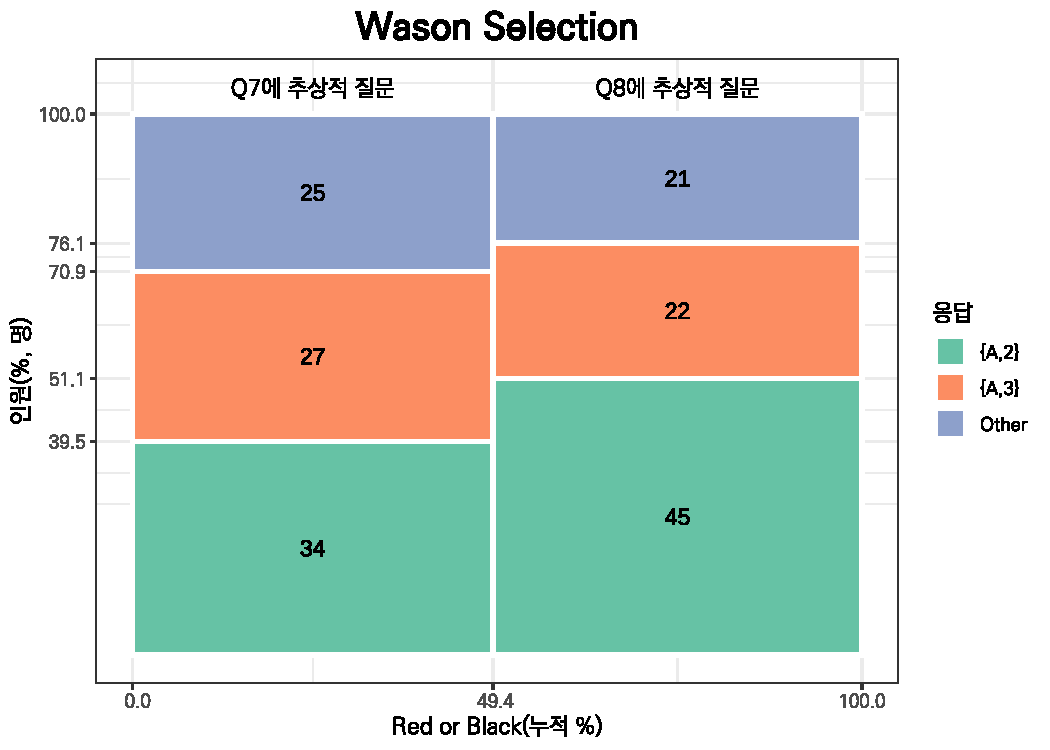
\includegraphics{quiz250414_Report_v4_files/figure-latex/mosaic plot_Q9-1.pdf}

Mosaic Plot으로부터 확증편향에서 비롯된 응답의 비율이 정답의 비율이나
기타 응답의 비율보다 월등히 높다는 것을 시각적으로 파악할 수 있습니다.

\subsection{학습 순서의
영향}\label{uxd559uxc2b5-uxc21cuxc11cuxc758-uxc601uxd5a5}

구체적 질문을 먼저 학습하고 추상적 질문을 학습하는 것과 추상적 질문을
먼저 학습하고 구체적 질문을 학습하는 방식 중에 어느 것이 더 나은지
비교한 결과 정답 인원은 매우 닮았는데, 순서에 따라 정답인원의 차이에는
통계적으로 유의한 차이가 관찰되지 않았습니다.

어떻게 해석할 수 있을까요?

\subsubsection{집계표}\label{uxc9d1uxacc4uxd45c}

\begin{longtable}[]{@{}
  >{\raggedright\arraybackslash}p{(\columnwidth - 6\tabcolsep) * \real{0.4110}}
  >{\centering\arraybackslash}p{(\columnwidth - 6\tabcolsep) * \real{0.2603}}
  >{\centering\arraybackslash}p{(\columnwidth - 6\tabcolsep) * \real{0.2603}}
  >{\centering\arraybackslash}p{(\columnwidth - 6\tabcolsep) * \real{0.0685}}@{}}
\caption{Wason Selection}\tabularnewline
\toprule\noalign{}
\begin{minipage}[b]{\linewidth}\raggedright
~
\end{minipage} & \begin{minipage}[b]{\linewidth}\centering
추상적 질문 정답
\end{minipage} & \begin{minipage}[b]{\linewidth}\centering
구체적 질문 정답
\end{minipage} & \begin{minipage}[b]{\linewidth}\centering
계
\end{minipage} \\
\midrule\noalign{}
\endfirsthead
\toprule\noalign{}
\begin{minipage}[b]{\linewidth}\raggedright
~
\end{minipage} & \begin{minipage}[b]{\linewidth}\centering
추상적 질문 정답
\end{minipage} & \begin{minipage}[b]{\linewidth}\centering
구체적 질문 정답
\end{minipage} & \begin{minipage}[b]{\linewidth}\centering
계
\end{minipage} \\
\midrule\noalign{}
\endhead
\bottomrule\noalign{}
\endlastfoot
\textbf{Red(추상적 질문 먼저)} & 29 & 55 & 84 \\
\textbf{Black(구체적 질문 먼저)} & 25 & 52 & 77 \\
\end{longtable}

\begin{longtable}[]{@{}
  >{\raggedleft\arraybackslash}p{(\columnwidth - 4\tabcolsep) * \real{0.2361}}
  >{\raggedleft\arraybackslash}p{(\columnwidth - 4\tabcolsep) * \real{0.0694}}
  >{\raggedleft\arraybackslash}p{(\columnwidth - 4\tabcolsep) * \real{0.1389}}@{}}
\caption{Pearson's Chi-squared test with Yates' continuity correction:
\texttt{.}}\tabularnewline
\toprule\noalign{}
\begin{minipage}[b]{\linewidth}\raggedleft
Test statistic
\end{minipage} & \begin{minipage}[b]{\linewidth}\raggedleft
df
\end{minipage} & \begin{minipage}[b]{\linewidth}\raggedleft
P value
\end{minipage} \\
\midrule\noalign{}
\endfirsthead
\toprule\noalign{}
\begin{minipage}[b]{\linewidth}\raggedleft
Test statistic
\end{minipage} & \begin{minipage}[b]{\linewidth}\raggedleft
df
\end{minipage} & \begin{minipage}[b]{\linewidth}\raggedleft
P value
\end{minipage} \\
\midrule\noalign{}
\endhead
\bottomrule\noalign{}
\endlastfoot
0.01187 & 1 & 0.9132 \\
\end{longtable}

추상적 질문을 Q7에 배치하고 구체적 질문을 Q8에 배치한 Red의 경우 추상적
질문과 구체적 질문에 정답을 올린 사람은 총 84(명)이고 구체적 질문을 Q7에
배치하고 추상적 질문을 Q8에 배치한 Black의 경우 추상적 질문과 구체적
질문에 정답을 올린 사람은 총 77(명)으로 별로 차이가 나지 않습니다.

추상적 질문을 Q8에 배치한 Black 의 경우 25(명) 이 정답을 올려서 추상적
질문을 먼저 학습한 경우 정답을 더 많이 내었지만 통계적으로 유의한 차이는
아닌 것으로 나타나고 있습니다.

카이제곱 통계량은 0.012, p-value 는 0.91으로 통계적으로 유의한 차이를
관찰하지 못하였습니다.

따라서 학습 순서는 추상적 질문의 정답율에 영향을 미치지 못하고 있습니다.

백분율을 살펴 보겠습니다.

\subsubsection{\% 비교}\label{uxbe44uxad50-1}

\begin{longtable}[]{@{}
  >{\raggedright\arraybackslash}p{(\columnwidth - 4\tabcolsep) * \real{0.4167}}
  >{\centering\arraybackslash}p{(\columnwidth - 4\tabcolsep) * \real{0.2639}}
  >{\centering\arraybackslash}p{(\columnwidth - 4\tabcolsep) * \real{0.2639}}@{}}
\caption{Wason Selection}\tabularnewline
\toprule\noalign{}
\begin{minipage}[b]{\linewidth}\raggedright
~
\end{minipage} & \begin{minipage}[b]{\linewidth}\centering
추상적 질문 정답
\end{minipage} & \begin{minipage}[b]{\linewidth}\centering
구체적 질문 정답
\end{minipage} \\
\midrule\noalign{}
\endfirsthead
\toprule\noalign{}
\begin{minipage}[b]{\linewidth}\raggedright
~
\end{minipage} & \begin{minipage}[b]{\linewidth}\centering
추상적 질문 정답
\end{minipage} & \begin{minipage}[b]{\linewidth}\centering
구체적 질문 정답
\end{minipage} \\
\midrule\noalign{}
\endhead
\bottomrule\noalign{}
\endlastfoot
\textbf{Red(추상적 질문 먼저)} & 53.7 & 51.4 \\
\textbf{Black(구체적 질문 먼저)} & 46.3 & 48.6 \\
\textbf{계} & 100.0 & 100.0 \\
\end{longtable}

추상적 질문에 대한 Red, Black 간 정답률 차이와 구체적 질문에 대한 Red,
Black 간 정답률 차이를 비교하였습니다.

추상적 질문에 대한 전체 정답 중에서 추상적 질문을 먼저 제시한 Red 가
53.7(\%)를 차지하여 추상적 질문을 나중에 제시한 Black 보다 높습니다만 그
차이는 앞에서 살펴 본 것처럼 통계적으로 유의하지는 않습니다.

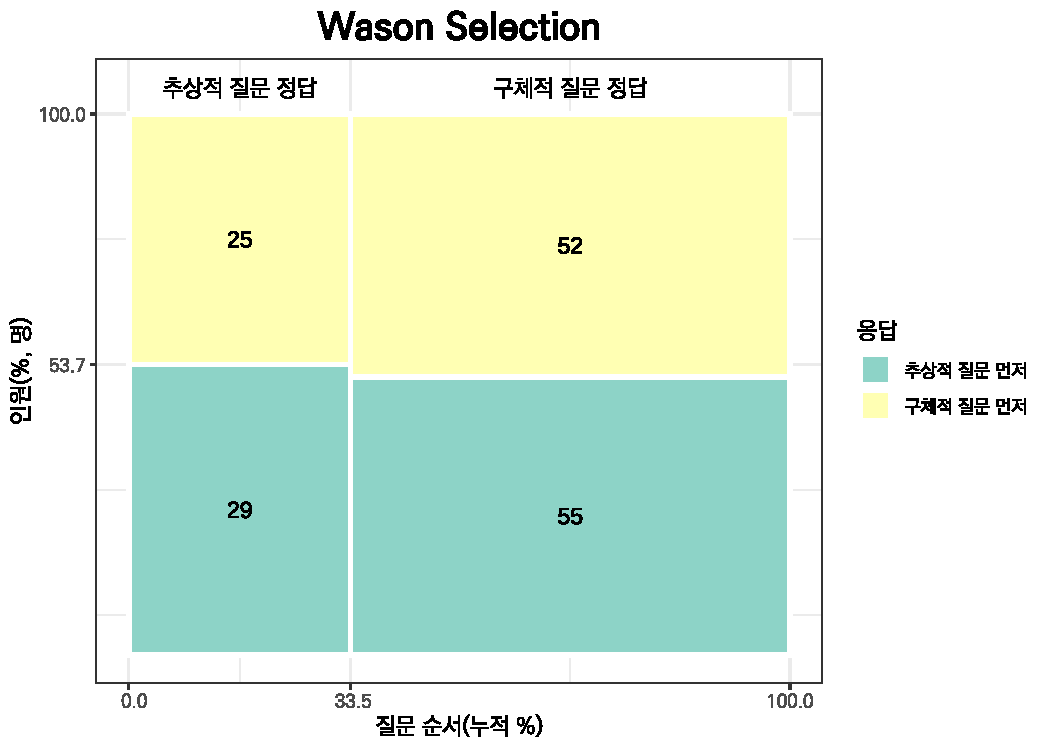
\includegraphics{quiz250414_Report_v4_files/figure-latex/mosaic plot3-1.pdf}

Mosaic Plot으로부터 구체적 질문이 먼저 주어진 Red나 구체적 질문이 나중에
주어진 Black이나정답을 올린 인원이나 백분율이 비슷한다는 것을 시각적으로
파악할 수 있습니다.

\subsubsection{합산}\label{uxd569uxc0b0}

실험에 참여한 어느 누구나 추상적 문제와 구체적 문제를 한 번씩 풀게
됩니다.

학습 순서의 영향은 없는 것으로 파악되었으니까 추상적 문제의 정답률과
구체적 문제의 정답률을 합쳐서 비교하는 것이 합리적입니다.

\subsubsection{집계표}\label{uxc9d1uxacc4uxd45c-1}

\begin{longtable}[]{@{}
  >{\raggedright\arraybackslash}p{(\columnwidth - 6\tabcolsep) * \real{0.2500}}
  >{\centering\arraybackslash}p{(\columnwidth - 6\tabcolsep) * \real{0.0972}}
  >{\centering\arraybackslash}p{(\columnwidth - 6\tabcolsep) * \real{0.0972}}
  >{\centering\arraybackslash}p{(\columnwidth - 6\tabcolsep) * \real{0.0972}}@{}}
\toprule\noalign{}
\begin{minipage}[b]{\linewidth}\raggedright
~
\end{minipage} & \begin{minipage}[b]{\linewidth}\centering
정답
\end{minipage} & \begin{minipage}[b]{\linewidth}\centering
오답
\end{minipage} & \begin{minipage}[b]{\linewidth}\centering
계
\end{minipage} \\
\midrule\noalign{}
\endhead
\bottomrule\noalign{}
\endlastfoot
\textbf{추상적 문제} & 54 & 120 & 174 \\
\textbf{구체적 문제} & 107 & 67 & 174 \\
\end{longtable}

추상적 질문에 답한 사람 총 174(명) 중에 정답을 올린 사람은 모두
54(명)이고 구체적 질문에 답한 사람 총 174(명) 중에 정답을 올린 사람은
모두 107(명)입니다. 백분율로 비교해 보면

\subsubsection{\% 비교}\label{uxbe44uxad50-2}

\begin{longtable}[]{@{}
  >{\raggedright\arraybackslash}p{(\columnwidth - 6\tabcolsep) * \real{0.2500}}
  >{\centering\arraybackslash}p{(\columnwidth - 6\tabcolsep) * \real{0.0972}}
  >{\centering\arraybackslash}p{(\columnwidth - 6\tabcolsep) * \real{0.0972}}
  >{\centering\arraybackslash}p{(\columnwidth - 6\tabcolsep) * \real{0.1111}}@{}}
\toprule\noalign{}
\begin{minipage}[b]{\linewidth}\raggedright
~
\end{minipage} & \begin{minipage}[b]{\linewidth}\centering
정답
\end{minipage} & \begin{minipage}[b]{\linewidth}\centering
오답
\end{minipage} & \begin{minipage}[b]{\linewidth}\centering
계
\end{minipage} \\
\midrule\noalign{}
\endhead
\bottomrule\noalign{}
\endlastfoot
\textbf{추상적 문제} & 31.0 & 69.0 & 100.0 \\
\textbf{구체적 문제} & 61.5 & 38.5 & 100.0 \\
\end{longtable}

추상적 질문에 정답을 올린 사람의 백분율은 31.0(\%)이고 구체적 질문에
정답을 올린 사람의 백분율은 31.0(\%)입니다.

추상적 질문의 정답율이 구체적 질문의 정답율에 비하여 월등히 낮다는 것을
알 수 있습니다. 이를 시각적으로 비교해 보겠습니다.

\subsubsection{Barplot}\label{barplot}


\includegraphics{quiz250414_Report_v4_files/figure-latex/unnamed-chunk-18-1.pdf}

이 경우에는 막대그래프로 표현하는 것이 보다 시각적으로 두 상황을
비교하기에 더 효과적입니다.

추상적 질문의 응답 중에서 정답의 비율이 구체적 질문의 응답 중 정답의
비율보다 월등히 적다는 것이 시각적으로 잘 드러나고 있습니다.

\subsection{마감 시간으로부터 제출 시간의
분포}\label{uxb9c8uxac10-uxc2dcuxac04uxc73cuxb85cuxbd80uxd130-uxc81cuxcd9c-uxc2dcuxac04uxc758-uxbd84uxd3ec}

\subsubsection{분포표}\label{uxbd84uxd3ecuxd45c}

\begin{longtable}[]{@{}
  >{\raggedright\arraybackslash}p{(\columnwidth - 30\tabcolsep) * \real{0.0863}}
  >{\raggedleft\arraybackslash}p{(\columnwidth - 30\tabcolsep) * \real{0.0576}}
  >{\raggedleft\arraybackslash}p{(\columnwidth - 30\tabcolsep) * \real{0.0576}}
  >{\raggedleft\arraybackslash}p{(\columnwidth - 30\tabcolsep) * \real{0.0576}}
  >{\raggedleft\arraybackslash}p{(\columnwidth - 30\tabcolsep) * \real{0.0576}}
  >{\raggedleft\arraybackslash}p{(\columnwidth - 30\tabcolsep) * \real{0.0576}}
  >{\raggedleft\arraybackslash}p{(\columnwidth - 30\tabcolsep) * \real{0.0576}}
  >{\raggedleft\arraybackslash}p{(\columnwidth - 30\tabcolsep) * \real{0.0576}}
  >{\raggedleft\arraybackslash}p{(\columnwidth - 30\tabcolsep) * \real{0.0576}}
  >{\raggedleft\arraybackslash}p{(\columnwidth - 30\tabcolsep) * \real{0.0576}}
  >{\raggedleft\arraybackslash}p{(\columnwidth - 30\tabcolsep) * \real{0.0647}}
  >{\raggedleft\arraybackslash}p{(\columnwidth - 30\tabcolsep) * \real{0.0719}}
  >{\raggedleft\arraybackslash}p{(\columnwidth - 30\tabcolsep) * \real{0.0719}}
  >{\raggedleft\arraybackslash}p{(\columnwidth - 30\tabcolsep) * \real{0.0719}}
  >{\raggedleft\arraybackslash}p{(\columnwidth - 30\tabcolsep) * \real{0.0719}}
  >{\centering\arraybackslash}p{(\columnwidth - 30\tabcolsep) * \real{0.0432}}@{}}
\caption{일 단위}\tabularnewline
\toprule\noalign{}
\begin{minipage}[b]{\linewidth}\raggedright
~
\end{minipage} & \begin{minipage}[b]{\linewidth}\raggedleft
{[}0,1{]}
\end{minipage} & \begin{minipage}[b]{\linewidth}\raggedleft
(1,2{]}
\end{minipage} & \begin{minipage}[b]{\linewidth}\raggedleft
(2,3{]}
\end{minipage} & \begin{minipage}[b]{\linewidth}\raggedleft
(3,4{]}
\end{minipage} & \begin{minipage}[b]{\linewidth}\raggedleft
(4,5{]}
\end{minipage} & \begin{minipage}[b]{\linewidth}\raggedleft
(5,6{]}
\end{minipage} & \begin{minipage}[b]{\linewidth}\raggedleft
(6,7{]}
\end{minipage} & \begin{minipage}[b]{\linewidth}\raggedleft
(7,8{]}
\end{minipage} & \begin{minipage}[b]{\linewidth}\raggedleft
(8,9{]}
\end{minipage} & \begin{minipage}[b]{\linewidth}\raggedleft
(9,10{]}
\end{minipage} & \begin{minipage}[b]{\linewidth}\raggedleft
(10,11{]}
\end{minipage} & \begin{minipage}[b]{\linewidth}\raggedleft
(11,12{]}
\end{minipage} & \begin{minipage}[b]{\linewidth}\raggedleft
(12,13{]}
\end{minipage} & \begin{minipage}[b]{\linewidth}\raggedleft
(13,14{]}
\end{minipage} & \begin{minipage}[b]{\linewidth}\centering
계
\end{minipage} \\
\midrule\noalign{}
\endfirsthead
\toprule\noalign{}
\begin{minipage}[b]{\linewidth}\raggedright
~
\end{minipage} & \begin{minipage}[b]{\linewidth}\raggedleft
{[}0,1{]}
\end{minipage} & \begin{minipage}[b]{\linewidth}\raggedleft
(1,2{]}
\end{minipage} & \begin{minipage}[b]{\linewidth}\raggedleft
(2,3{]}
\end{minipage} & \begin{minipage}[b]{\linewidth}\raggedleft
(3,4{]}
\end{minipage} & \begin{minipage}[b]{\linewidth}\raggedleft
(4,5{]}
\end{minipage} & \begin{minipage}[b]{\linewidth}\raggedleft
(5,6{]}
\end{minipage} & \begin{minipage}[b]{\linewidth}\raggedleft
(6,7{]}
\end{minipage} & \begin{minipage}[b]{\linewidth}\raggedleft
(7,8{]}
\end{minipage} & \begin{minipage}[b]{\linewidth}\raggedleft
(8,9{]}
\end{minipage} & \begin{minipage}[b]{\linewidth}\raggedleft
(9,10{]}
\end{minipage} & \begin{minipage}[b]{\linewidth}\raggedleft
(10,11{]}
\end{minipage} & \begin{minipage}[b]{\linewidth}\raggedleft
(11,12{]}
\end{minipage} & \begin{minipage}[b]{\linewidth}\raggedleft
(12,13{]}
\end{minipage} & \begin{minipage}[b]{\linewidth}\raggedleft
(13,14{]}
\end{minipage} & \begin{minipage}[b]{\linewidth}\centering
계
\end{minipage} \\
\midrule\noalign{}
\endhead
\bottomrule\noalign{}
\endlastfoot
\textbf{Red} & 0 & 0 & 0 & 0 & 0 & 0 & 0 & 0 & 0 & 16 & 12 & 16 & 18 &
24 & 86 \\
\textbf{Black} & 0 & 0 & 0 & 0 & 0 & 0 & 0 & 0 & 1 & 14 & 11 & 14 & 16 &
32 & 88 \\
\textbf{계} & 0 & 0 & 0 & 0 & 0 & 0 & 0 & 0 & 1 & 30 & 23 & 30 & 34 & 56
& 174 \\
\end{longtable}

분포표로부터 두 가지 문제를 살펴보겠습니다.

첫째, 날마다 고르게 제출하는가?

둘째, Red, Black 간에 통계적으로 유의한 차이가 있는가?

각 문제를 살펴보기 위해서는 분포표의 일부분을 대상으로 카이제곱 테스트를
수행합니다.

\subsubsection{날마다 고르게
제출하는가?}\label{uxb0a0uxb9c8uxb2e4-uxace0uxb974uxac8c-uxc81cuxcd9cuxd558uxb294uxac00}

\begin{longtable}[]{@{}
  >{\raggedleft\arraybackslash}p{(\columnwidth - 10\tabcolsep) * \real{0.1111}}
  >{\raggedleft\arraybackslash}p{(\columnwidth - 10\tabcolsep) * \real{0.1250}}
  >{\raggedleft\arraybackslash}p{(\columnwidth - 10\tabcolsep) * \real{0.1389}}
  >{\raggedleft\arraybackslash}p{(\columnwidth - 10\tabcolsep) * \real{0.1389}}
  >{\raggedleft\arraybackslash}p{(\columnwidth - 10\tabcolsep) * \real{0.1389}}
  >{\raggedleft\arraybackslash}p{(\columnwidth - 10\tabcolsep) * \real{0.1389}}@{}}
\toprule\noalign{}
\begin{minipage}[b]{\linewidth}\raggedleft
(8,9{]}
\end{minipage} & \begin{minipage}[b]{\linewidth}\raggedleft
(9,10{]}
\end{minipage} & \begin{minipage}[b]{\linewidth}\raggedleft
(10,11{]}
\end{minipage} & \begin{minipage}[b]{\linewidth}\raggedleft
(11,12{]}
\end{minipage} & \begin{minipage}[b]{\linewidth}\raggedleft
(12,13{]}
\end{minipage} & \begin{minipage}[b]{\linewidth}\raggedleft
(13,14{]}
\end{minipage} \\
\midrule\noalign{}
\endhead
\bottomrule\noalign{}
\endlastfoot
1 & 30 & 23 & 30 & 34 & 56 \\
\end{longtable}

\begin{longtable}[]{@{}
  >{\raggedleft\arraybackslash}p{(\columnwidth - 4\tabcolsep) * \real{0.2361}}
  >{\raggedleft\arraybackslash}p{(\columnwidth - 4\tabcolsep) * \real{0.0694}}
  >{\raggedleft\arraybackslash}p{(\columnwidth - 4\tabcolsep) * \real{0.2361}}@{}}
\caption{Chi-squared test for given probabilities:
\texttt{.}}\tabularnewline
\toprule\noalign{}
\begin{minipage}[b]{\linewidth}\raggedleft
Test statistic
\end{minipage} & \begin{minipage}[b]{\linewidth}\raggedleft
df
\end{minipage} & \begin{minipage}[b]{\linewidth}\raggedleft
P value
\end{minipage} \\
\midrule\noalign{}
\endfirsthead
\toprule\noalign{}
\begin{minipage}[b]{\linewidth}\raggedleft
Test statistic
\end{minipage} & \begin{minipage}[b]{\linewidth}\raggedleft
df
\end{minipage} & \begin{minipage}[b]{\linewidth}\raggedleft
P value
\end{minipage} \\
\midrule\noalign{}
\endhead
\bottomrule\noalign{}
\endlastfoot
54.34 & 5 & 1.78e-10 * * * \\
\end{longtable}

날마다 고르게 제출하는지 알아 보았습니다.

분포표의 ``계''행에서 '계'열을 제외하고 카이제곱테스트를 수행합니다.

분포표 만으로도 쉽게 파악할 수 있지만 카이제곱테스트가 명확히 해 줍니다.

카이제곱 통계량은 54.34, 자유도는 5.00, p-value 는 1.8e-10 이므로
아직까지는 날짜별로 고르게 제출하고 있습니다.

막대그래프로 살펴 보겠습니다.

\subsubsection{막대그래프}\label{uxb9c9uxb300uxadf8uxb798uxd504}

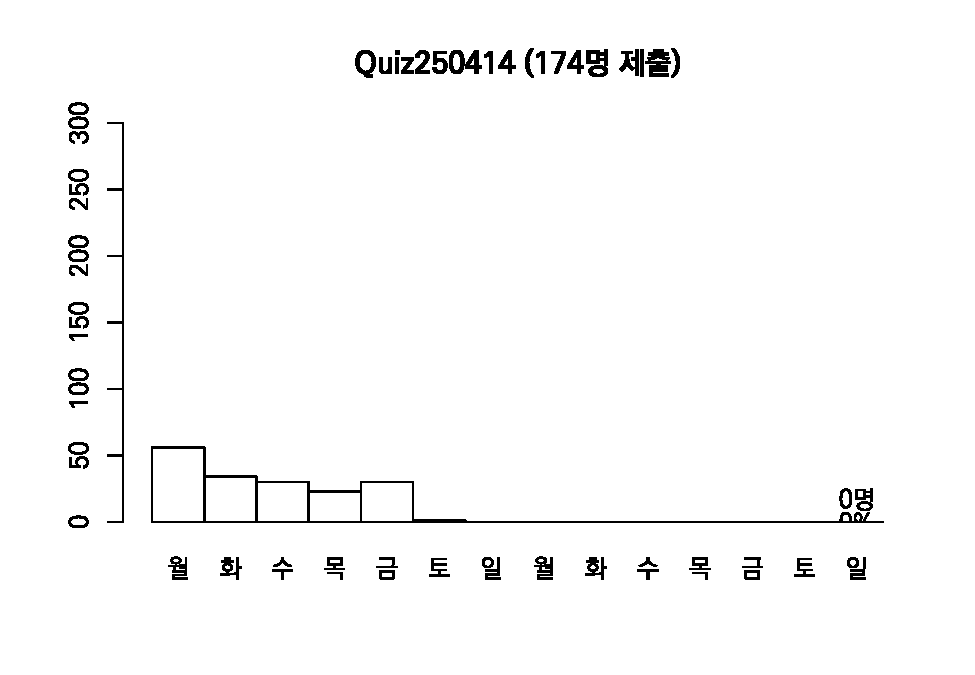
\includegraphics{quiz250414_Report_v4_files/figure-latex/unnamed-chunk-21-1.pdf}

\subsubsection{Red, Black 간에
닮았는가?}\label{red-black-uxac04uxc5d0-uxb2eeuxc558uxb294uxac00}

\begin{longtable}[]{@{}
  >{\raggedright\arraybackslash}p{(\columnwidth - 12\tabcolsep) * \real{0.1667}}
  >{\raggedleft\arraybackslash}p{(\columnwidth - 12\tabcolsep) * \real{0.1111}}
  >{\raggedleft\arraybackslash}p{(\columnwidth - 12\tabcolsep) * \real{0.1250}}
  >{\raggedleft\arraybackslash}p{(\columnwidth - 12\tabcolsep) * \real{0.1389}}
  >{\raggedleft\arraybackslash}p{(\columnwidth - 12\tabcolsep) * \real{0.1389}}
  >{\raggedleft\arraybackslash}p{(\columnwidth - 12\tabcolsep) * \real{0.1389}}
  >{\raggedleft\arraybackslash}p{(\columnwidth - 12\tabcolsep) * \real{0.1389}}@{}}
\toprule\noalign{}
\begin{minipage}[b]{\linewidth}\raggedright
~
\end{minipage} & \begin{minipage}[b]{\linewidth}\raggedleft
(8,9{]}
\end{minipage} & \begin{minipage}[b]{\linewidth}\raggedleft
(9,10{]}
\end{minipage} & \begin{minipage}[b]{\linewidth}\raggedleft
(10,11{]}
\end{minipage} & \begin{minipage}[b]{\linewidth}\raggedleft
(11,12{]}
\end{minipage} & \begin{minipage}[b]{\linewidth}\raggedleft
(12,13{]}
\end{minipage} & \begin{minipage}[b]{\linewidth}\raggedleft
(13,14{]}
\end{minipage} \\
\midrule\noalign{}
\endhead
\bottomrule\noalign{}
\endlastfoot
\textbf{Red} & 0 & 16 & 12 & 16 & 18 & 24 \\
\textbf{Black} & 1 & 14 & 11 & 14 & 16 & 32 \\
\end{longtable}

\begin{longtable}[]{@{}
  >{\raggedleft\arraybackslash}p{(\columnwidth - 4\tabcolsep) * \real{0.2361}}
  >{\raggedleft\arraybackslash}p{(\columnwidth - 4\tabcolsep) * \real{0.0694}}
  >{\raggedleft\arraybackslash}p{(\columnwidth - 4\tabcolsep) * \real{0.1389}}@{}}
\caption{Pearson's Chi-squared test: \texttt{.}}\tabularnewline
\toprule\noalign{}
\begin{minipage}[b]{\linewidth}\raggedleft
Test statistic
\end{minipage} & \begin{minipage}[b]{\linewidth}\raggedleft
df
\end{minipage} & \begin{minipage}[b]{\linewidth}\raggedleft
P value
\end{minipage} \\
\midrule\noalign{}
\endfirsthead
\toprule\noalign{}
\begin{minipage}[b]{\linewidth}\raggedleft
Test statistic
\end{minipage} & \begin{minipage}[b]{\linewidth}\raggedleft
df
\end{minipage} & \begin{minipage}[b]{\linewidth}\raggedleft
P value
\end{minipage} \\
\midrule\noalign{}
\endhead
\bottomrule\noalign{}
\endlastfoot
2.548 & 5 & 0.7692 \\
\end{longtable}

제출시간의 분포가 Red, Black 간에 닮았는지 알아 보았습니다.

이번에는 분포표의 첫번째와 두번째 행, '계'열을 제외한 나머지 열에 대해서
카이제곱테스트를 수행합니다.

카이제곱 통계량은 2.55, 자유도는 5, p-value 는 0.7692 이므로 제출 시간의
분포는 Red, Black 간에 통계적으로 유의한 차이가 관찰되지 않습니다.

이 사실을 Mosaic Plot 을 이용하여 시각적으로 살펴보겠습니다.

닮았다고 느껴지나요?

\subsubsection{Mosaic Plot}\label{mosaic-plot-3}

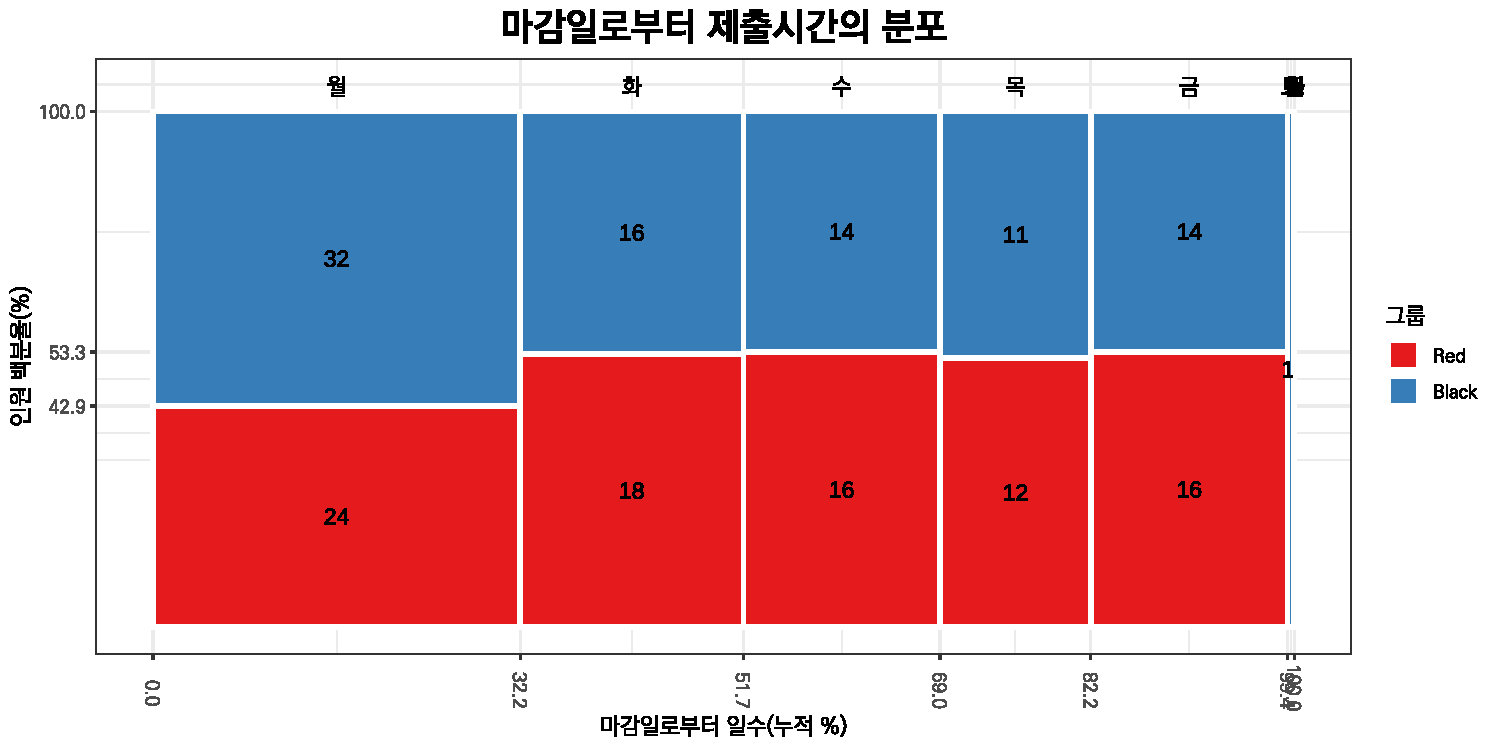
\includegraphics{quiz250414_Report_v4_files/figure-latex/unnamed-chunk-23-1.pdf}

\end{document}
